%\documentclass[draft]{ua-thesis}
\documentclass[final]{ua-thesis}
%<my packages>
%% Language and font encodings
\usepackage{gb4e}
\noautomath
\usepackage{natbib}
\usepackage[english]{babel}
\usepackage[utf8x]{inputenc}
\usepackage[T1]{fontenc}

%% Sets page size and margins
%\usepackage[a4paper,top=3cm,bottom=2cm,left=3cm,right=3cm,marginparwidth=1.75cm]{geometry}

%% Useful packages
\usepackage{amsmath}
\usepackage{graphicx}
\usepackage[colorinlistoftodos]{todonotes}
\usepackage[colorlinks=true, allcolors=blue]{hyperref}
\usepackage{fixltx2e}
\usepackage{rotating}
\usepackage{Sweave}

\newcommand*{\myfont}{\fontfamily{ccr}\selectfont}
%the newcommand change the selected word into 'ccr' font
%e.g. \begin{myfont} multi-bleu.perl \end{myfont}
%<\my packages>
%packages used by Koeh
\usepackage{url}
\usepackage{color}
\usepackage{epic,ecltree}
\usepackage{eclbip}
\usepackage{multicol}
\usepackage{algorithmic}
\usepackage{algorithm}
\renewcommand{\algorithmicrequire}{\textbf{Input:}}
\renewcommand{\algorithmicensure}{\textbf{Output:}}
\renewcommand{\algorithmiccomment}[1]{// {\em #1}}

\definecolor{darkblue}{rgb}{0,0,0.8}
\definecolor{darkgreen}{rgb}{0,0.8,0}
\definecolor{reddishgreen}{rgb}{0.4,0.6,0}
\definecolor{purple}{rgb}{0.6,0,0.6}
\definecolor{red}{rgb}{1,0,0}

\newcommand{\example}[1]{\textcolor{darkblue}{\rm #1}}
\newcommand{\maths}[1]{\textcolor{purple}{#1}}
\newcommand{\reference}[1]{\vspace{-2mm}\begin{flushright}\textcolor{purple}{\tiny [from #1]}\end{flushright}\vspace{-7mm}}
%End packages used by Koeh

\usepackage{verbatim}
%\usepackage{amssymb,amsmath,amsthm}
%\usepackage[mathscr]{eucal}

\usepackage{makeidx}
\numberwithin{equation}{section}
%\numberwithin{equation}{subsection}
%%====================================================================
%-------------------------------------------------------------------- 
%
%   isomath.tex  LaTeX macros for math conforming to ISO standards
%
%---------------------------------------- this is a LaTeX-2e document
%====================================================================     

%% Blackboard Bold

\newcommand*{\bbb}[1]{\mathbb{#1}}
\newcommand{\bC}{\bbb{C}}
\newcommand{\bN}{\bbb{N}}
\newcommand{\bQ}{\bbb{Q}}
\newcommand{\bR}{\bbb{R}}
\newcommand{\bZ}{\bbb{Z}}
\newcommand{\bF}{\bbb{F}}
\newcommand{\bFp}{\bbb{F}_p}
\newcommand{\bFpn}{\bbb{F}_{p^n}}
\newcommand{\ii}{\mathbf{i}}
\newcommand{\jj}{\mathbf{j}}
\newcommand{\kk}{\mathbf{k}}

\newcommand{\N}{\bN}
\newcommand{\Q}{\bQ}
\newcommand{\R}{\bR}
\newcommand{\Z}{\bZ}
\newcommand{\ZpZ}{\Z/p\Z}
\newcommand{\ZmZ}{\Z/m\Z}
\newcommand{\C}{\bC}
%\newcommand{\F}{\bF}
\newcommand{\F}{\mathbb{F}}
\newcommand{\Fp}{\bFp}
\newcommand{\Fpn}{\bFpn}

%% Calligraphic

\newcommand{\mC}{\mathcal{C}}
\newcommand{\mT}{\mathcal{T}}

%% Miscellaneous

%% Named Functions and Operators

\newcommand{\id}{\mathrm{id}}
\newcommand{\Id}{\mathrm{Id}}
\newcommand{\rank}{\mathrm{rank}}
\newcommand{\supp}{\mathrm{supp}}
\newcommand{\tr}{\mathrm{tr}}
\newcommand{\Aut}{\mathrm{Aut}}
\newcommand{\Gal}{\mathrm{Gal}}
\newcommand{\Hom}{\mathrm{Hom}}
\newcommand{\im}{\mathrm{im}}
\newcommand{\lcm}{\mathrm{lcm}}
\newcommand{\Tr}{\mathrm{Tr}}
\newcommand{\GL}{\mathrm{GL}}
%\newcommand{\mod}{\textrm{ mod }}

%% Vectors

\usepackage{amsbsy}
\renewcommand*{\vec}[1]{\boldsymbol{#1}}
\newcommand{\va}{\vec{a}}
\newcommand{\vb}{\vec{b}}
\newcommand{\vc}{\vec{c}}
\newcommand{\vx}{\vec{x}}
\newcommand{\vy}{\vec{y}}
\newcommand{\vz}{\vec{z}}
\newcommand{\vu}{\vec{u}}
\newcommand{\vv}{\vec{v}}
\newcommand{\vw}{\vec{w}}

%% Logical Propositions

\newcommand*{\pro}[1]{\mathsf{#1}}
\newcommand{\pP}{\pro{P}}
\newcommand{\pQ}{\pro{Q}}
\newcommand{\pR}{\pro{R}}

%% Matrices and Tensors

%\DeclareMathAlphabet{\mathsfsl}{OT1}{cmss}{m}{sl}
\newcommand*{\mat}[1]{\mathsfsl{#1}}
\newcommand{\mM}{\mat{M}}
\newcommand{\mD}{\mat{D}}
\newcommand{\mI}{\mat{I}}

%% Special Numbers and Characters

\newcommand{\re}{\mathrm{e}}
\newcommand{\ri}{\mathrm{i}}
\newcommand{\rd}{\mathrm{d}} % differential
\newcommand{\dif}[1]{\,\rd{#1}} % differential
\newcommand{\df}{\dif{f}}
\newcommand{\dx}{\dif{x}}
\newcommand{\dy}{\dif{y}}
\newcommand{\dz}{\dif{z}}
\newcommand{\dt}{\dif{t}}
\newcommand{\rpi}{\pi}       % actually, pi should be upright.

\newcommand{\rE}{\mathsf{E}}
\newcommand{\rF}{\mathsf{F}}
\newcommand{\rI}{\mathsf{I}}
\newcommand{\rK}{\mathsf{K}}
\newcommand{\rL}{\mathsf{L}}
\newcommand{\rM}{\mathsf{M}}
\newcommand{\rN}{\mathsf{N}}
\newcommand{\rP}{\mathsf{P}}
\newcommand{\rT}{\mathsf{T}}
\newcommand{\rU}{\mathsf{U}}
\newcommand{\rV}{\mathsf{V}}
\newcommand{\rW}{\mathsf{W}}
\newcommand{\rX}{\mathsf{X}}
\newcommand{\rY}{\mathsf{Y}}
\newcommand{\rZ}{\mathsf{Z}}

%====================================================================
%
%  mathenv.tex  math environments  version 0.00
%
%====================================================================

\usepackage{ifthen}

\theoremstyle{plain}
%\newtheorem{thm}{Theorem}[subsection]
\newtheorem{thm}[equation]{Theorem}
\newtheorem{cor}[equation]{Corollary}
\newtheorem{lem}[equation]{Lemma}
\newtheorem{prop}[equation]{Proposition}
\newtheorem{ax}[equation]{Axiom}
\newtheorem*{thm*}{Theorem}
\newtheorem*{cor*}{Corollary}
\newtheorem*{lem*}{Lemma}
\newtheorem*{prop*}{Proposition}
\newtheorem*{ax*}{Axiom}

\theoremstyle{definition}
\newtheorem{defn}[equation]{Definition}
\newtheorem{problem}{Problem}
\newtheorem*{defn*}{Definition}
\newtheorem*{problem*}{Problem}
% \newtheorem{ex}[equation]{Example}
% \newtheorem{exs}[equation]{Examples}
% \newtheorem*{ex*}{Example}
% \newtheorem*{exs*}{Examples}

%\theoremstyle{remark}
\newtheorem{rem}[equation]{Remark}
\newtheorem*{rem*}{Remark}
\newtheorem{aside}[equation]{Aside}
\newtheorem*{aside*}{Aside}
\newtheorem{intuition}[equation]{Intuition}
\newtheorem*{intuition*}{Intuition}
\newtheorem{notn}[equation]{Notation}
\newtheorem*{notn*}{Notation}
\newtheorem{conv}[equation]{Convention}
\newtheorem*{conv*}{Convention}
\newtheorem{interp}[equation]{Interpretation}
\newtheorem*{interp*}{Interpretation}
\newtheorem{mnem}[equation]{Mnemonic}
\newtheorem*{mnem*}{Mnemonic}
\newtheorem{exer}[equation]{Exercise}
\newtheorem*{exer*}{Exercise}
\newtheorem{conjecture}[equation]{Conjecture}
\newtheorem*{conjecture*}{Conjecture}

%\numberwithin{equation}{subsection}
%\numberwithin{equation}{section}

%\newcommand{\beginex}{\begin{ex}$\blacktriangleright$ }
%\newcommand{\mendex}{\hfill$\blacktriangleleft$\end{ex}}
\newcommand{\beginex}{\begin{ex}$\rhd$ }
\newcommand{\mendex}{\hfill$\lhd$\end{ex}}

%--------------------------------------------------------------------
%
%\newenvironment{problem}[1][]
% {\noindent{\bf#1.\ }}
% {}
%
%--------------------------------------------------------------------

\newenvironment{answer}[1][Answer]
  {\begin{proof}[#1]}
  {\renewcommand{\qedsymbol}{}\end{proof}}

\newenvironment{solution}[1][Solution]
  {\begin{proof}[#1]}
  {\renewcommand{\qedsymbol}{\ensuremath{\Diamond}}\end{proof}}

\newcounter{ppart}
\newenvironment{parts}
 {\begin{list}{\textup(\alph{ppart}\textup)\hfill}
   {\usecounter{ppart}
    \settowidth{\labelwidth}{\textup(m\textup)}
    \setlength{\leftmargin}{0cm} 
    \setlength{\rightmargin}{0cm}
    \setlength{\itemindent}{2em}
    \setlength{\labelsep}{\itemindent}
    \addtolength{\labelsep}{-\labelwidth}
    \renewcommand{\makelabel}[1]{\ifthenelse
     {\equal{##1}{}}
     {\textup{(\alph{ppart})}\hfill}
     {\textup{##1}\hfill}}
   }
 }
 {\end{list}}

%\renewcommand{\labelenumi}{(\roman{enumi})}

\newcommand{\secref}[1]{Section~\textup{\ref{#1}}}
\newcommand{\thmref}[1]{Theorem~\textup{\ref{#1}}}
\newcommand{\corref}[1]{Corollary~\textup{\ref{#1}}}
\newcommand{\lemref}[1]{Lemma~\textup{\ref{#1}}}
\newcommand{\propref}[1]{Proposition~\textup{\ref{#1}}}
\newcommand{\defnref}[1]{Definition~\textup{\ref{#1}}}
\newcommand{\remref}[1]{Remark~\textup{\ref{#1}}}
\newcommand{\exref}[1]{Example~\textup{\ref{#1}}}
\newcommand{\exsref}[1]{Examples~\textup{\ref{#1}}}
\newcommand{\axref}[1]{Axiom~\textup{\ref{#1}}}
\newcommand{\itemref}[1]{\textup{{\ref{#1}}}}

% Vim 7.0 syntax highlighting doesn't seem to kick in unless the .tex
% file has at least one begin-end pair in it.  Go figure.
\newenvironment{vim_bug_workaround}
	{}

%====================================================================


\newcommand*{\ds}[1]{\displaystyle{#1}}

\newcommand*{\bfidx}[1]{\index{#1}\textbf{#1}}
\newcommand*{\bfidxtwo}[2]{\textbf{#1}\index{#2}}
\newcommand*{\bfidxaux}[2]{\index{#1}\index{#2}\textbf{#1}}
\newcommand*{\emphidx}[1]{\index{#1}\emph{#1}}
\newcommand*{\plainidx}[1]{\index{#1}#1}

\newcommand*{\bra}[1]{\langle \, #1 \mid}
\newcommand*{\ket}[1]{\mid #1 \, \rangle}
\newcommand*{\braket}[2]{\langle #1 \mid #2 \rangle}
\newcommand*{\braCket}[3]{\langle #1 \mid #2 \mid #3 \rangle}
\newcommand*{\BraCKet}[3]
	{\Bigg\langle #1 \,\Bigg|\, #2 \,\Bigg|\, #3 \Bigg\rangle}
\newcommand*{\expn}[1]{\langle \, #1 \, \rangle}
\newcommand*{\ketbra}[1]{\ket{ #1 } \bra{ #1 }}
\newcommand*{\TrebH}{\Tr\left(e^{-\beta H}\right)}
\newcommand*{\TrXebH}[1]{\Tr\left(#1 e^{-\beta H}\right)}
\newcommand*{\Trsym}{\Tr_{L^2_{\mathrm{sym}}}}
\newcommand*{\intRdntimes}[2]{\underbrace{
	\int_{\R^{#1}} \int_{\R^{#1}} \cdots \int_{\R^{#1}}}_{#2 \textrm{ times}}}

\newcommand{\lmax}{\ell_{\textrm{max}}}

\newcommand{\ellx}{\ell_{\vecx}}
\newcommand{\elly}{\ell_{\vecy}}

\newcommand{\ellxpi}{\ell_{\vecx}(\pi)}
\newcommand{\ellypi}{\ell_{\vecy}(\pi)}

\newcommand{\ellxpiprime}{\ell_{\vecx}(\pi')}
\newcommand{\ellypiprime}{\ell_{\vecy}(\pi')}

\newcommand{\ellxypi}{\ell_{\vecx,\vecy}(\pi)}
\newcommand{\ellyxpi}{\ell_{\vecy,\vecx}(\pi)}

\newcommand{\essx}{s_{\vecx}}

\newcommand{\essxpi}{s_{\vecx}(\pi)}

\newcommand{\ellxf}{\ell^f_{\vecx}}
\newcommand{\essxf}{s^f_{\vecx}}
\newcommand{\ellmax}{\ell_{\textrm{max}}}
\newcommand{\fM}{f_{\textrm{max}}}
\newcommand{\ellbar}{\overline{\ell}}
\newcommand{\ellfbar}{\overline{\ell}_f}
\newcommand{\essbar}{\overline{s}}
\newcommand{\essfbar}{\overline{s}_f}

\newcommand{\rhocz}{\rho_c^{(0)}}
\newcommand{\rhocal}{\rho_c^{(\alpha)}}
\newcommand{\betacz}{\beta_c^{(0)}}
\newcommand{\betacal}{\beta_c^{(\alpha)}}
\newcommand{\Tcz}{T_c^{(0)}}
\newcommand{\Tcal}{T_c^{(\alpha)}}

\newcommand{\Xt}{X_t}
\newcommand{\Yt}{Y_t}
\newcommand{\Xtk}{X_{t+k}}
\newcommand{\Ytk}{Y_{t+k}}

\newcommand{\cmhat}{\hat{c}_m}
\newcommand{\chat}{\hat{c}}
\newcommand{\tauint}{{\tau_{\textrm{int}}}}
\newcommand{\hattauint}{\hat{\tau}_{\textrm{int}}}
\newcommand{\tauexp}{{\tau_{\textrm{exp}}}}
\newcommand{\stilde}{{\tilde{s}}}
\newcommand{\ttilde}{{\tilde{t}}}

\newcommand{\sumiB}{\sum_{i=0}^{B-1}}
\newcommand{\sumjB}{\sum_{j=0}^{B-1}}
\newcommand{\sumiM}{\sum_{i=0}^{M-1}}
\newcommand{\sumjM}{\sum_{j=0}^{M-1}}
\newcommand{\sumiN}{\sum_{i=0}^{N-1}}
\newcommand{\sumjN}{\sum_{j=0}^{N-1}}

%% ----------------------------------------------------------------
\def\ve{\varepsilon}
\def\veps{\varepsilon}
\def\bbB{\mathbb{B}}
\def\bbE{\mathbb{E}}
\def\bbP{\mathbb{P}}
\def\muhat{\hat{\mu}}
\def\psihat{\hat{\psi}}
\def\fhat{\hat{f}}
\def\ghat{\hat{g}}
\def\Ahat{\hat{A}}
\def\Fhat{\hat{F}}
\def\Hhat{\hat{H}}
\def\What{\hat{W}}
\def\Yhat{\hat{Y}}
\def\Zhat{\hat{Z}}
\def\nuhat{\hat{\nu}}
\def\rhohat{\hat{\rho}}
\def\Xihat{\hat{Xi}}
\def\xbar{\overline{x}}
%\def\torusdiff{\tilde{\vecd}}
\def\torusdiff{\vecd_\Lambda}

\def\muX{\mu_{X}}
\def\muY{\mu_{Y}}
\def\muXNbar{\mu_{\overline{X}_N}}
\def\muYNbar{\mu_{\overline{Y}_N}}
\def\sigmaX{\sigma_{X}}
\def\sigmaY{\sigma_{Y}}
\def\sigmaXNbar{\sigma_{\overline{X}_N}}
\def\sigmaYNbar{\sigma_{\overline{Y}_N}}

\def\ANbar{{\overline{A}_N}}

\def\QMbar{{\overline{Q}_M}}

\def\Xbar{\overline{X}}
\def\XNbar{{\overline{X}_N}}
\def\XMbar{{\overline{X}_M}}
\def\XNBbar{{\overline{X}_{N,B}}}

\def\Ybar{\overline{Y}}
\def\YNbar{\overline{Y}_N}
\def\YNBbar{\overline{Y}_{N,B}}

\def\Z{\mathbb{Z}}

\def\Htilde{\tilde{H}}
\def\Halpha{H^{(\alpha)}}
\def\HP{H_P}
\def\HPzero{H_P^{(0)}}
\def\HPone{H_P^{(1)}}

\def\bfH{\mathbf{H}}
\def\bfx{\mathbf{x}}

\def\bsH{\mathbf{H}}
\def\bsx{\mathbf{x}}

\def\caS{\mathcal{S}}
\def\mcS{\mathcal{S}}

\def\mcF{\mathcal{F}}
\def\mcK{\mathcal{K}}
\def\mcL{\mathcal{L}}
\def\mcH{\mathcal{H}}
\def\mcN{\mathcal{N}}
\def\mcO{\mathcal{O}}

\def\msH{\mathscr{H}}
\newcommand*{\pig}[1]{\langle #1 \rangle}
\newcommand*{\pigm}[1]{\langle #1 \rangle_M}

%% ----------------------------------------------------------------
\newcommand{\Sn}{\mathcal{S}_n}
\newcommand{\SN}{\mathcal{S}_N}
\newcommand{\SNp}{\mathcal{S}_{N+1}}
\newcommand{\SNpc}{{\SNp \setminus \SN}}
\newcommand{\dd}{\mathrm{d}}
\newcommand{\e}{\mathrm{e}}
\newcommand{\Var}{\mathrm{Var}}
\newcommand{\Corr}{\mathrm{Corr}}
\newcommand{\Cov}{\mathrm{Cov}}

%% ----------------------------------------------------------------
\def\veca{\mathbf{a}}
\def\vecb{\mathbf{b}}
\def\vecc{\mathbf{c}}
\def\vecd{\mathbf{d}}
\def\vecg{\mathbf{g}}
\def\veck{\mathbf{k}}
\def\vecm{\mathbf{m}}
\def\vecn{\mathbf{n}}
\def\vecr{\mathbf{r}}
\def\vecu{\mathbf{u}}
\def\vecv{\mathbf{v}}
\def\vecw{\mathbf{w}}
\def\vecx{\mathbf{x}}
\def\vecy{\mathbf{y}}
\def\vecz{\mathbf{z}}

\def\vecK{\mathbf{K}}
\def\vecM{\mathbf{M}}
\def\vecP{\mathbf{P}}
%\def\vecP{\mathcal{P}}
\def\vecV{\mathbf{V}}
\def\vecW{\mathbf{W}}
\def\vecWhat{\hat{\mathbf{W}}}
\def\vecX{\mathbf{X}}
\def\vecY{\mathbf{Y}}
\def\vecZ{\mathbf{Z}}

\def\vecPpiz{\vecP^{(\pi_0)}}
\def\Ppiz{P^{(\pi_0)}}
\def\P{P_{\mathrm{Gibbs}}}
\def\Phat{\hat{P}_{\mathrm{Gibbs}}}

%\def\mkvM{\mathbf{M}}
%\def\mkvM{R}
\def\mkvM{A}
%\def\mkvM{\mathcal{M}}

\newcommand{\vecomega}{{\boldsymbol{\omega}}}
\newcommand{\vecmu}{{\boldsymbol{\mu}}}
\newcommand{\vecnu}{{\boldsymbol{\nu}}}

\def\vecxi{\mathbf{x}_{i}}
\def\vecxj{\mathbf{x}_{j}}
\def\vecxpii{\mathbf{x}_{\pi(i)}}
\def\vecxpij{\mathbf{x}_{\pi(j)}}
\def\vecxpik{\mathbf{x}_{\pi(k)}}
\def\veckpii{\mathbf{k}_{\pi(i)}}

\def\pii{\pi^{-1}}
\def\piinv{\pi^{-1}}

\def\pix{\pi(\vecx)}
\def\piy{\pi(\vecy)}

\def\piprimex{\pi'(\vecx)}
\def\piprimey{\pi'(\vecy)}

\def\piv{\pi(\vecv)}
\def\piw{\pi(w)}
\def\piiw{\pi^{-1}(w)}
\def\piix{\pi^{-1}(\vecx)}
\def\piiy{\pi^{-1}(\vecy)}
\def\edh{e^{-\Delta H}}

\def\vecwi{\mathbf{w}^{(i)}}
\def\vecwj{\mathbf{w}^{(j)}}
\def\vecwk{\mathbf{w}^{(k)}}
\def\vecwij{\mathbf{w}^{(ij)}}

\def\vecwil{\mathbf{w}^{(i_\ell)}}
\def\vecwjl{\mathbf{w}^{(j_\ell)}}

\def\xhat{\hat{x}}
\def\yhat{\hat{y}}

\DeclareMathOperator*{\ctdto}{\circ\hspace{-0.2mm}--\hspace{-0.3mm}\circ}
\DeclareMathOperator*{\notctdto}{\circ\hspace{-0.2mm}--\hspace{-2.5mm}\not--\hspace{-0.3mm}\circ}
\def\maybeeq{\stackrel{?}{=}}
\DeclareMathOperator*{\twocyc}{\circ\hspace{-0.2mm}-\pi-\hspace{-0.4mm}\circ}
\DeclareMathOperator*{\ntwocyc}{\circ\hspace{-0.2mm}-\not\pi-\hspace{-0.4mm}\circ}


%% ----------------------------------------------------------------
\newcommand{\tand}{\textrm{and}}
\newcommand{\qand}{\quad\textrm{and}\quad}
\newcommand{\qqand}{\qquad\textrm{and}\qquad}
\newcommand{\qor}{\quad\textrm{or}\quad}
\newcommand{\qqor}{\qquad\textrm{or}\qquad}
\newcommand{\qie}{\quad\textrm{i.e.}\quad}
\newcommand{\qqie}{\qquad\textrm{i.e.}\qquad}
\newcommand{\qqwith}{\qquad\textrm{with}\qquad}

%% ================================================================
%\newcommand{\Suto}{S\"ut\H{o}}
\def\Suto{S\"ut\H{o}}

\newcommand{\grad}{\nabla}
\newcommand{\tensor}{\otimes}
\newcommand{\into}{\hookrightarrow}
\newcommand{\longto}{\longrightarrow}
\def\upto{\nearrow}
\newcommand{\ix}{\pi(x)}
\newcommand{\iy}{\pi^{-1}(y)}
\newcommand{\iu}{\pi(u)}
\newcommand{\tat}{\textasciitilde}

\newcommand*{\boxalign}[1]{
	\begin{equation*}
	\addtolength{\fboxsep}{5pt}
	\boxed{
	\begin{aligned}
	#1
	\end{aligned}
	}
	\end{equation*}
}

\newcommand*{\rowvectwo}[2]{\begin{pmatrix}#1 & #2 \end{pmatrix}}
\newcommand*{\rowvecthree}[3]{\begin{pmatrix}#1 & #2 & #3\end{pmatrix}}

\newcommand*{\colvecone}[1]{\left(\begin{array}{r} #1 \end{array}\right)}
\newcommand*{\colvectwo}[2]{\left(\begin{array}{r} #1 \\ #2 \end{array}\right)}
\newcommand*{\colvecthree}[3]{\left(\begin{array}{r} #1 \\ #2 \\ #3\end{array}\right)}
\newcommand*{\colvecfour}[4]{\left(\begin{array}{r} #1 \\ #2 \\ #3 \\ #4\end{array}\right)}

\newcommand*{\collvecone}[1]{\left(\begin{array}{l} #1 \end{array}\right)}
\newcommand*{\collvectwo}[2]{\left(\begin{array}{l} #1 \\ #2 \end{array}\right)}
\newcommand*{\collvecthree}[3]{\left(\begin{array}{l} #1 \\ #2 \\ #3\end{array}\right)}
\newcommand*{\collvecfour}[4]{\left(\begin{array}{l} #1 \\ #2 \\ #3 \\ #4\end{array}\right)}

\newcommand*{\colcvecone}[1]{\left(\begin{array}{c} #1 \end{array}\right)}
\newcommand*{\colcvectwo}[2]{\left(\begin{array}{c} #1 \\ #2 \end{array}\right)}
\newcommand*{\colcvecthree}[3]{\left(\begin{array}{c} #1 \\ #2 \\ #3\end{array}\right)}
\newcommand*{\colcvecfour}[4]{\left(\begin{array}{c} #1 \\ #2 \\ #3 \\ #4\end{array}\right)}

\newcommand*{\colrvecone}[1]{\left(\begin{array}{r} #1 \end{array}\right)}
\newcommand*{\colrvectwo}[2]{\left(\begin{array}{r} #1 \\ #2 \end{array}\right)}
\newcommand*{\colrvecthree}[3]{\left(\begin{array}{r} #1 \\ #2 \\ #3\end{array}\right)}
\newcommand*{\colrvecfour}[4]{\left(\begin{array}{r} #1 \\ #2 \\ #3 \\ #4\end{array}\right)}

%% ----------------------------------------------------------------
\newcommand{\D}{\partial}
\newcommand{\DA}{\partial A}
\newcommand{\DB}{\partial B}
\newcommand{\DC}{\partial C}
\newcommand{\DX}{\partial X}
\newcommand{\Dc}{\partial c}
\newcommand{\Df}{\partial f}
\newcommand{\Dg}{\partial g}
\newcommand{\DG}{\partial G}
\newcommand{\Dh}{\partial h}
\newcommand{\DM}{\partial M}
\newcommand{\Dr}{\partial r}
\newcommand{\Du}{\partial u}
\newcommand{\Dx}{\partial x}
\newcommand{\Dy}{\partial y}
\newcommand{\Dz}{\partial z}
\newcommand{\Ds}{\partial s}
\newcommand{\Dt}{\partial t}

\newcommand{\DD}{\partial/\partial}
\newcommand{\DDA}{\partial/\partial A}
\newcommand{\DDB}{\partial/\partial B}
\newcommand{\DDC}{\partial/\partial C}
\newcommand{\DDX}{\partial/\partial X}
\newcommand{\DDc}{\partial/\partial c}
\newcommand{\DDf}{\partial/\partial f}
\newcommand{\DDg}{\partial/\partial g}
\newcommand{\DDG}{\partial/\partial G}
\newcommand{\DDh}{\partial/\partial h}
\newcommand{\DDM}{\partial/\partial M}
\newcommand{\DDr}{\partial/\partial r}
\newcommand{\DDx}{\partial/\partial x}
\newcommand{\DDy}{\partial/\partial y}
\newcommand{\DDz}{\partial/\partial z}
\newcommand{\DDs}{\partial/\partial s}
\newcommand{\DDt}{\partial/\partial t}

%% ----------------------------------------------------------------
\newcommand*{\slashD}[1]{\partial/\partial #1}
\newcommand*{\fracD}[1]{\frac{\partial}{\partial #1}}
\newcommand*{\slashDtwo}[2]{\partial #1/\partial #2}
\newcommand*{\fracDtwo}[2]{\frac{\partial #1}{\partial #2}}

\newcommand{\slashDx}{\partial/\partial x}
\newcommand{\slashDy}{\partial/\partial y}
\newcommand{\slashDz}{\partial/\partial z}

\newcommand{\fracDs}{\frac{\partial}{\partial s}}
\newcommand{\fracDt}{\frac{\partial}{\partial t}}
\newcommand{\fracDx}{\frac{\partial}{\partial x}}
\newcommand{\fracDy}{\frac{\partial}{\partial y}}
\newcommand{\fracDz}{\frac{\partial}{\partial z}}
\newcommand{\fracDxx}{\frac{\partial^2}{\partial x^2}}

\newcommand{\fracDfx}{\frac{\partial f}{\partial x}}
\newcommand{\fracDfy}{\frac{\partial f}{\partial y}}
\newcommand{\fracDfz}{\frac{\partial f}{\partial z}}

\newcommand{\fracDgt}{\frac{\partial g}{\partial t}}
\newcommand{\fracDgu}{\frac{\partial g}{\partial u}}
\newcommand{\fracDguu}{\frac{\partial^2 g}{\partial u^2}}
\newcommand{\fracDgv}{\frac{\partial g}{\partial v}}
\newcommand{\fracDgvv}{\frac{\partial^2 g}{\partial v^2}}
\newcommand{\fracDguv}{\frac{\partial^2 g}{\partial u \partial v}}

\newcommand{\fracDht}{\frac{\partial h}{\partial t}}
\newcommand{\fracDhu}{\frac{\partial h}{\partial u}}
\newcommand{\fracDhuu}{\frac{\partial^2 h}{\partial u^2}}
\newcommand{\fracDhv}{\frac{\partial h}{\partial v}}
\newcommand{\fracDhvv}{\frac{\partial^2 h}{\partial v^2}}
\newcommand{\fracDhuv}{\frac{\partial^2 h}{\partial u \partial v}}

\newcommand{\fracDgx}{\frac{\partial g}{\partial x}}
\newcommand{\fracDgxx}{\frac{\partial^2 g}{\partial x^2}}
\newcommand{\fracDgy}{\frac{\partial g}{\partial y}}
\newcommand{\fracDgyy}{\frac{\partial^2 g}{\partial y^2}}
\newcommand{\fracDgz}{\frac{\partial g}{\partial z}}
\newcommand{\fracDgxy}{\frac{\partial^2 g}{\partial x \partial y}}

\newcommand{\fracDhx}{\frac{\partial h}{\partial x}}
\newcommand{\fracDhxx}{\frac{\partial^2 h}{\partial x^2}}
\newcommand{\fracDhy}{\frac{\partial h}{\partial y}}
\newcommand{\fracDhyy}{\frac{\partial^2 h}{\partial y^2}}
\newcommand{\fracDhz}{\frac{\partial h}{\partial z}}
\newcommand{\fracDhxy}{\frac{\partial^2 h}{\partial x \partial y}}

\newcommand{\fracDphis}{\frac{\partial    \phi}{\partial s}}
\newcommand{\fracDphit}{\frac{\partial    \phi}{\partial t}}
\newcommand{\fracDphix}{\frac{\partial    \phi}{\partial x}}
\newcommand{\fracDphixx}{\frac{\partial^2 \phi}{\partial x^2}}
\newcommand{\fracDphiy}{\frac{\partial    \phi}{\partial y}}
\newcommand{\fracDphiyy}{\frac{\partial^2 \phi}{\partial y^2}}
\newcommand{\fracDphiz}{\frac{\partial    \phi}{\partial z}}
\newcommand{\fracDphixy}{\frac{\partial^2 \phi}{\partial x \partial y}}

\newcommand{\fracDxDy}{\frac{\partial x}{\partial y}}
\newcommand{\fracDxDz}{\frac{\partial x}{\partial z}}
\newcommand{\fracDyDx}{\frac{\partial y}{\partial x}}
\newcommand{\fracDyDz}{\frac{\partial y}{\partial z}}
\newcommand{\fracDzDx}{\frac{\partial z}{\partial x}}
\newcommand{\fracDzDy}{\frac{\partial z}{\partial y}}

\newcommand{\fracDfDx}{\frac{\partial f}{\partial x}}
\newcommand{\fracDfDy}{\frac{\partial f}{\partial y}}
\newcommand{\fracDfDz}{\frac{\partial f}{\partial z}}

\newcommand{\slashDxDy}{\partial x/\partial y}
\newcommand{\slashDxDz}{\partial x/\partial z}
\newcommand{\slashDyDx}{\partial y/\partial x}
\newcommand{\slashDyDz}{\partial y/\partial z}
\newcommand{\slashDzDx}{\partial z/\partial x}
\newcommand{\slashDzDy}{\partial z/\partial y}

\newcommand{\slashDfDx}{\partial f/\partial x}
\newcommand{\slashDfDy}{\partial f/\partial y}
\newcommand{\slashDfDz}{\partial f/\partial z}

%% ----------------------------------------------------------------
% Parenthesized matrix with left alignment.
\newcommand*{\plmatrix}[1]{
	\left(\begin{array}{llllllllllll}
		#1
	\end{array}\right)
}

% Parenthesized matrix with centered alignment.
\newcommand*{\pcmatrix}[1]{
	\left(\begin{array}{cccccccccccc}
		#1
	\end{array}\right)
}

% Parenthesized matrix with right alignment.
\newcommand*{\prmatrix}[1]{
	\left(\begin{array}{rrrrrrrrrrrr}
		#1
	\end{array}\right)
}

%% ----------------------------------------------------------------
% Bracketed matrix with left alignment.
\newcommand*{\blmatrix}[1]{
	\left[\begin{array}{llllllllllll}
		#1
	\end{array}\right]
}

% Bracketed matrix with centered alignment.
\newcommand*{\bcmatrix}[1]{
	\left[\begin{array}{cccccccccccc}
		#1
	\end{array}\right]
}

% Bracketed matrix with right alignment.
\newcommand*{\brmatrix}[1]{
	\left[\begin{array}{rrrrrrrrrrrr}
		#1
	\end{array}\right]
}

%% ----------------------------------------------------------------
% Unbracketed matrix with left alignment.
\newcommand*{\nlmatrix}[1]{
	\begin{array}{llllllllllll}
		#1
	\end{array}
}

% Unbracketed matrix with centered alignment.
\newcommand*{\ncmatrix}[1]{
	\begin{array}{cccccccccccc}
		#1
	\end{array}
}

% Unbracketed matrix with right alignment.
\newcommand*{\nrmatrix}[1]{
	\begin{array}{rrrrrrrrrrrr}
		#1
	\end{array}
}

\usepackage{graphicx}
\usepackage{psfrag}
\usepackage{afterpage}
\usepackage{subfigure}
\usepackage{hyperref}
\usepackage{ifpdf}
\usepackage{qtree}
\usepackage{fixltx2e}
\graphicspath{ {figures/} }
\DeclareMathOperator*{\argmax}{argmax} 
\usepackage{tikz}
\usetikzlibrary{matrix,chains,positioning,decorations.pathreplacing,arrows}
\usetikzlibrary {positioning}

\usetikzlibrary{fit,positioning,arrows.meta}
\tikzset{
  neuron/.style={ % style for each neuron
    circle,draw,thick, % drawn as a thick circle
    inner sep=0pt, % no built-in padding between the text and the circle shape
    minimum size=3.5em, % make each neuron the same size regardless of the text inside
    node distance=1ex and 2em, % spacing between neurons (y and x)
  },
  group/.style={ % style for the groups of neurons
    rectangle,draw,thick, % drawn as a thick rectangle
    inner sep=0pt, % no padding between the node contents and the rectangle shape
  },
  io/.style={ % style for the inputs/outputs
    neuron, % inherit the neuron style
    fill=gray!15, % add a fill color
  },
  conn/.style={ % style for the connections
    -{Straight Barb[angle=60:2pt 3]}, % simple barbed arrow tip
    thick, % draw in a thick weight to match other drawing elements
  },
}


\director{Mike Hammond}


\author{Yuan-Lu Chen}
\title{Improving Neural Net Machine Translation Systems with Linguistic Information}
\date{2018}
\makeindex

\ifpdf
\pdfinfo{
/Author (Yuan-Lu Chen)
/Title  (Improving Neural Net Machine Translation Systems with Linguistic Information)
}
\fi

%% ================================================================
\begin{document}
\Sconcordance{concordance:RealMaster.tex:RealMaster.Rnw:%
1 132 1}
\Sconcordance{concordance:RealMaster.tex:./Introduction.Rnw:ofs 133:%
1 13 1}
\Sconcordance{concordance:RealMaster.tex:./gloss.Rnw:ofs 147:%
1 279 1}
\Sconcordance{concordance:RealMaster.tex:RealMaster.Rnw:ofs 427:%
136}
\Sconcordance{concordance:RealMaster.tex:./intro_MT.Rnw:ofs 428:%
1 178 1}
\Sconcordance{concordance:RealMaster.tex:./Perceptron_fig.Rnw:ofs 607:%
1 48 1}
\Sconcordance{concordance:RealMaster.tex:./intro_MT.Rnw:ofs 656:%
181 27 1}
\Sconcordance{concordance:RealMaster.tex:./neural_network_hidden_fig.Rnw:ofs 684:%
1 46 1}
\Sconcordance{concordance:RealMaster.tex:./intro_MT.Rnw:ofs 731:%
210 13 1}
\Sconcordance{concordance:RealMaster.tex:./rnn_figure.Rnw:ofs 745:%
1 44 1}
\Sconcordance{concordance:RealMaster.tex:./intro_MT.Rnw:ofs 790:%
225 76 1}
\Sconcordance{concordance:RealMaster.tex:./RealCake.Rnw:ofs 867:%
1 231 1}
\Sconcordance{concordance:RealMaster.tex:./GLOSS_table.Rnw:ofs 1099:%
1 1 17 23 0}
\Sconcordance{concordance:RealMaster.tex:./RealCake.Rnw:ofs 1124:%
234 19 1}
\Sconcordance{concordance:RealMaster.tex:./RealCake2.Rnw:ofs 1144:%
1 80 1}
\Sconcordance{concordance:RealMaster.tex:./ParaPart_table.Rnw:ofs 1225:%
1 1 17 23 0}
\Sconcordance{concordance:RealMaster.tex:./RealCake2.Rnw:ofs 1250:%
83 38 1}
\Sconcordance{concordance:RealMaster.tex:./Para_table.Rnw:ofs 1289:%
1 1 17 23 0}
\Sconcordance{concordance:RealMaster.tex:./RealCake2.Rnw:ofs 1314:%
123}
\Sconcordance{concordance:RealMaster.tex:./GDParaParaPart_null_table.Rnw:ofs 1315:%
1}
\Sconcordance{concordance:RealMaster.tex:./RealCake2.Rnw:ofs 1316:%
125 2 1}
\Sconcordance{concordance:RealMaster.tex:./GDParaParaPart_table.Rnw:ofs 1319:%
1 1 19 23 0}
\Sconcordance{concordance:RealMaster.tex:./RealCake2.Rnw:ofs 1344:%
129 28 1}
\Sconcordance{concordance:RealMaster.tex:./interleavingGdGLOSS_table.Rnw:ofs 1373:%
1 1 17 23 0}
\Sconcordance{concordance:RealMaster.tex:./RealCake2.Rnw:ofs 1398:%
159 23 1}
\Sconcordance{concordance:RealMaster.tex:./concat_table.Rnw:ofs 1422:%
1 1 17 23 0}
\Sconcordance{concordance:RealMaster.tex:./RealCake2.Rnw:ofs 1447:%
184 36 1}
\Sconcordance{concordance:RealMaster.tex:./ReplacingGaelic_table.Rnw:ofs 1484:%
1 1 17 23 0}
\Sconcordance{concordance:RealMaster.tex:./RealCake2.Rnw:ofs 1509:%
222 3 1}
\Sconcordance{concordance:RealMaster.tex:./ReplacingGLOSS_table.Rnw:ofs 1513:%
1 1 17 23 0}
\Sconcordance{concordance:RealMaster.tex:./RealCake2.Rnw:ofs 1538:%
227 9 1 1 11 23 0 1 2 12 1}
\Sconcordance{concordance:RealMaster.tex:./Tying_loose_ends.Rnw:ofs 1585:%
1 15 1}
\Sconcordance{concordance:RealMaster.tex:./google_table.Rnw:ofs 1601:%
1 1 17 23 0}
\Sconcordance{concordance:RealMaster.tex:./Tying_loose_ends.Rnw:ofs 1626:%
18 25 1}
\Sconcordance{concordance:RealMaster.tex:./over_table.Rnw:ofs 1652:%
1 1 17 23 0}
\Sconcordance{concordance:RealMaster.tex:./Tying_loose_ends.Rnw:ofs 1677:%
45 5 1}
\Sconcordance{concordance:RealMaster.tex:./HyPara_table.Rnw:ofs 1683:%
1 1 6 33 0}
\Sconcordance{concordance:RealMaster.tex:./Tying_loose_ends.Rnw:ofs 1718:%
52 15 1}
\Sconcordance{concordance:RealMaster.tex:./Other_language_table.Rnw:ofs 1734:%
1 1 26 29 0}
\Sconcordance{concordance:RealMaster.tex:./Tying_loose_ends.Rnw:ofs 1765:%
69 12 1}
\Sconcordance{concordance:RealMaster.tex:./Conclusion_and_Future_Research.Rnw:ofs 1778:%
1 37 1}
\Sconcordance{concordance:RealMaster.tex:RealMaster.Rnw:ofs 1816:%
142 6 1}


\maketitle

\chapter*{Dedication}
\thispagestyle{topright}
\begin{center}For Eva, the best linguist and the most powerful neual machine.\end{center}
\chapter*{Acknowledgments}
acknowledgment!
Many people help me and keep me company in my this journey.
Thank you.

\begin{vim_bug_workaround}
\end{vim_bug_workaround}


\tableofcontents
\listoffigures
\listoftables

\begin{abstract}
Interlinear Glossed Text is widely used in linguistic studies. The following is an example of Scottish Gaelic Interlinear Glossed Text.
\begin{exe}  
\exi{(i)} \gll    Tha a athair nas sine na a mh\`athair.\\  
            be.pres 3sm.poss father comp old.cmpr comp 3sm.poss mother
\\  
    \glt    `His father is older than his mother.'  
\end{exe}

In a simple form of Interlinear Glossed Text, the first line is a sentence of the language of interest, the second line is a word-by-word translation, annotated with relevant grammatical information, and the third line is an English translation.  

The Innovation of the current work is to incorporate the gloss information of Interlinear Glossed Text data into neural net machine translation systems.
 
Critically, if the Gaelic data and the gloss data are combined in a specific way as the training data, I term which as Parallel-Partial treatment, the performance of the systems is improved significantly. The Parallel-Partial treatment lets machine to learn four sets of mappings: 1.) from source sentence to target sentence, 2) from gloss lines to target sentences, 3) from gloss lines to source sentences, and 4) from source language words to gloss items. 

Moreover, the boosting effect of the Parallel-Partial treatment is consistent across different languages and across neural net machine translation systems with different hyper-parameter settings. 

How theoretical linguistics may work hand in hand with natural language processing, and how neural net machine learning may exploit linguistics are important questions. \citet{pater2017generative}. The current work also exemplifies how theoretical linguistics may work hand in hand with natural language processing successfully, in addition to practically building better machine translation systems.   
\end{abstract}

%%% ================================================================
\chapter{Chapter title}
\label{chap:one_chapter}

%% ----------------------------------------------------------------
\section{Disclaimers and usage instructions}

This is a version of my PhD dissertation which I defended and got through
Graduate College format review in spring 2010.  I hope it works for you.
Please keep in mind, however, that style policies may change.  Of course,
please consult the style information you received from the Graduate College.

I should acknowledge that I didn't write this from scratch.  I got this
template from I forget where --- somewhere in LPL, I think --- and modified to
my taste, and to match current formatting requirements.  So, this is a current
snapshot of collectively developed dissertation style for the University
of Arizona.

How to use this template:

\begin{itemize}

\item Search around in
\texttt{stu-dent-dis.tex},
\texttt{ua-thesis.cls},
\texttt{disack.tex}, etc. for the names ``Stuart Dent'' and
``Anna Mehmbuhr'', etc.  Change these to your name and the names of your
committee members.  Also change the title of your dissertation.

\item In those same files, look for anything else which needs changing.

\item In the first line of \texttt{stu-dent-dis.tex}, you can set the style to
\texttt{draft} or \texttt{final}.

\item The shell scripts \texttt{./dbuild} and \texttt{./pbuild}, in the
same directory as this file, can be used to create DVI and PDF files,
respectively.

\item Any {\LaTeX} problem you have is most likely resolvable by a Google
search.

\item Good luck, and have fun!

\end{itemize}

--- John ``Stu Dent'' Kerl, April 21, 2010.

%% ----------------------------------------------------------------
\section{Section title}
\label{sec:a_section}

The quick brown \plainidx{fox} jumped over the lazy \plainidx{dogs}.
The quick brown fox jumped over the lazy dogs.
The quick brown fox jumped over the lazy dogs.
The quick brown fox jumped over the lazy dogs.
The quick brown fox jumped over the lazy dogs.
The quick brown fox jumped over the lazy dogs.
The quick brown fox jumped over the lazy dogs.
The quick brown fox jumped over the lazy dogs.
The quick brown fox jumped over the lazy dogs.
The quick brown fox jumped over the lazy dogs.
The quick brown fox jumped over the lazy dogs.
The quick brown \emphidx{fox} jumped over the lazy dogs.

Table \ref{table:quadratic_data} will be discussed in section
\ref{sec:another_section}.

\begin{table}[thb]
$$
\begin{tabular}{|c|c|}
\hline $x$ & $f(x)$ \\
\hline
\hline $0$   &  $0$ \\
\hline $1$   &  $1$ \\
\hline $2$   &  $4$ \\
\hline $3$   &  $9$ \\
\hline $4$   & $16$ \\
\hline $5$   & $25$ \\
\hline
\end{tabular}
$$
\caption[Short caption for the list of tables.]
	{Here is the long caption for the body of the document.  Note that it's OK
	for this to have many lines.  But the short caption for the list of tables
	should be short.  Hence the difference between square brackets and curly
	braces in the \texttt{caption} command in the {\LaTeX} code.  And, you
	guessed it --- this last sentence is here just to make this caption even
	longer.
	\label{table:quadratic_data}}
\end{table}

%% ----------------------------------------------------------------
\section{Section title}
\label{sec:another_section}

\begin{table}[thb]
$$
\begin{tabular}{|c|c|}
\hline $x$ & $g(x)$ \\
\hline
\hline $0$   &   $0$ \\
\hline $1$   &   $1$ \\
\hline $2$   &   $8$ \\
\hline $3$   &  $27$ \\
\hline $4$   &  $64$ \\
\hline $5$   & $125$ \\
\hline
\end{tabular}
$$
\caption
	{Here is another caption.
	\label{table:cubic_data}}
\end{table}

The quick brown fox jumped over the lazy dogs.
The quick brown fox jumped over the lazy dogs.
The quick brown \plainidx{fox} jumped over the lazy \plainidx{dogs}.
The quick brown fox jumped over the lazy dogs.
The quick brown fox jumped over the lazy dogs.
The quick brown fox jumped over the lazy dogs.
The quick brown fox jumped over the lazy dogs.
The quick brown fox jumped over the lazy dogs.
The quick brown fox jumped over the lazy dogs.
The quick brown fox jumped over the lazy dogs.
The quick brown fox jumped over the lazy dogs.
The quick brown fox jumped over the lazy dogs.
The quick brown fox jumped over the lazy dogs.
The quick brown fox jumped over the lazy dogs.

Compare table \ref{table:cubic_data} with table \ref{table:quadratic_data}
which was on page \pageref{table:quadratic_data}.  We conjecture, but
are unable to prove, a relationship between these tabular data and
the function of equation \eqref{eqn:conjecture}:
\begin{align}
\label{eqn:conjecture}
	y &= x^4 - x^2 + 1.
\end{align}

%% ================================================================
\chapter{Chapter title}
\label{chap:another_chapter}

The quick brown fox jumped over the lazy dogs.
The quick brown fox jumped over the lazy dogs.
The quick brown fox jumped over the lazy dogs.
The quick brown fox jumped over the lazy dogs.
The quick brown fox jumped over the lazy dogs.
The quick brown fox jumped over the lazy dogs.
The quick brown fox jumped over the lazy dogs.
The quick brown fox jumped over the lazy dogs.
The quick brown fox jumped over the lazy dogs.
The quick brown fox jumped over the lazy dogs.
The quick brown fox jumped over the lazy dogs.
The quick brown fox jumped over the lazy dogs.
The quick brown fox jumped over the lazy dogs.

Please see figure \ref{fig:important}.

\begin{figure}[!htb]
\begin{center}
\psfragscanon
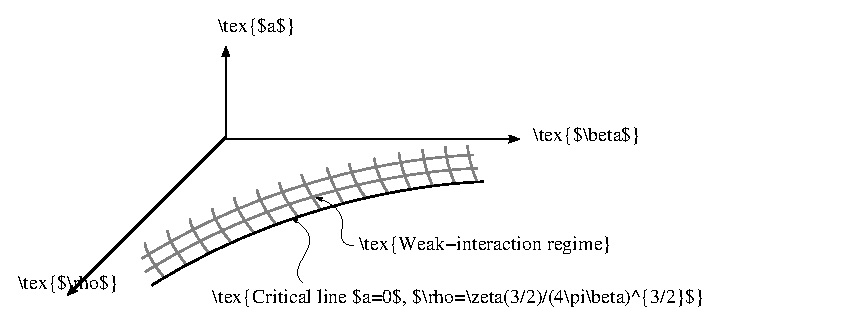
\includegraphics{figures/critical_manifold.eps}
\caption[Short caption for the list of figures.]
	{Here is an EPS file which I put in here and which surely must be
	important.
	\label{fig:important}}
\end{center}
\end{figure}

%% ----------------------------------------------------------------
\section{Section title}
\label{sec:yet_another_section}

The quick brown fox jumped over the lazy dogs.
The quick brown fox jumped over the lazy dogs.
The quick brown fox jumped over the lazy dogs.
The quick brown fox jumped over the lazy dogs.
The quick brown fox jumped over the lazy dogs.
The quick brown \emphidx{fox} jumped over the lazy \emphidx{dogs}.
The quick brown fox jumped over the lazy dogs.
The quick brown fox jumped over the lazy dogs.
The quick brown fox jumped over the lazy dogs.
The quick brown fox jumped over the lazy dogs.
The quick brown fox jumped over the lazy dogs.
The quick brown fox jumped over the lazy dogs.
The quick brown fox jumped over the lazy dogs.

%% ----------------------------------------------------------------
\section{Section title}
\label{sec:last_section}

The quick brown fox jumped over the lazy dogs.
The quick brown fox jumped over the lazy dogs.
The quick brown fox jumped over the lazy dogs.
The quick brown fox jumped over the lazy dogs.
The quick brown fox jumped over the lazy dogs.
The quick brown fox jumped over the lazy dogs.
The quick brown fox jumped over the lazy dogs.
The quick brown fox jumped over the lazy dogs.
The quick brown \plainidx{fox} jumped over the lazy \plainidx{dogs}.
The quick brown fox jumped over the lazy dogs.
The quick brown fox jumped over the lazy dogs.
The quick brown fox jumped over the lazy dogs.
The quick brown fox jumped over the lazy dogs.


\printindex

\chapter{Introduction}
\label{chap:Introduction}
\setcounter{exx}{0}
The fundamental argument that I am trying to make in the dissertation is follows:

\begin{exe}
	\ex Without linguistics, we only have ordinary natural language processing systems. With linguistics, we have extraordinary natural language processing systems. 
\end{exe}

Specifically, the curious question is whether or not interlinear glossed texts, a everyday tool for linguistic studies, can help machine translation. 
The following is an example interlinear glossed text:

\begin{exe}  
\ex\label{gloss_eg} Indonesian \citep[p. 237]{sneddon2012indonesian}
	\gll   Mereka di Jakarta sekarang. (\textit{sentence of interest})\\
     	   they in Jakarta now (\textit{gloss line: word-by-word gloss translation})\\
    \glt   `The are in Jakarta now.' (\textit{English translation})  
\end{exe}

The first line in an interlinear glossed text is the sentence of interest in its written form, the second line is a word by word morpheme by morpheme translation, and the third line is the corresponding English translation. 

The glossing data has very interesting properties. First, it contains linguistics information. The glosses are not raw natural data, but are already processed by linguists based the linguistic theory he or she adopts. Second, it is a type of big data, because interlinear glossed texts are so widely used in linguistics.
Both natural language processing and linguistics are studying human languages. Gloss is the right `lingua franca' for the two fields. 

Also thanks to the advent of neural net sequence to sequence machine learning, which is a generic algorithm that can learn almost any sequence to sequence mapping, the chance to successful incorporate the gloss line into machine translation is also better than other past time.  

With high expectations on the gloss line information, I conducted a series of machine translation experiments. It is found that the gloss information is an very effective booster for neural net machine translation systems in all conditions. 

The rest of the dissertation is organized as follows: chapter 2 discusses the nature of gloss lines, and argues that they are proper representations of meanings; chapter 3 provides a general overview of machine learning and machine translation; chapter 4, chapter 5 and chapter 6 are a series of neural net machine translation experiments; chapter 7 outlines potential future researches and concludes the dissertation.  
\chapter{What are glosses? Why are they golden representations of meanings?}
\label{chap:gloss}

\section{Introduction: What are Glosses?}

Interlinear Glossed Text is widely used in linguistic studies. The following is an example of Interlinear Glossed Text.
\begin{exe}  
\ex\label{gloss_eg} Indonesian \citep[p. 237]{sneddon2012indonesian}
	\gll   Mereka di Jakarta sekarang. (\textit{sentence of interest})\\
     	   they in Jakarta now (\textit{gloss line: word-by-word gloss translation})\\
    \glt   `The are in Jakarta now.' (\textit{English translation})  
\end{exe}

A chunk of an interlinear glossed text has three lines. The first line is the sentence of interest. The second line is the gloss line, which is a word-by-word translation of the first line. And the third line a free English translation of the first line.

The conventional way to show the word-by-word translation from the first line to the gloss line is to use vertical alignment. In (\ref{gloss_eg}), `\textit{Mereka}' is glossed as `\textit{they}', `\textit{di}' is glossed as `\textit{in}', `\textit{Jakarta}' is glossed as `\textit{Jakarta}', and `\textit{sekarang}' is glossed as `\textit{now}'. These pairs are vertically aligned. 

The gloss line also provides morphological information. Consider the following example:

\begin{exe}  
\ex French
	\gll   aux chevaux\\
     	   to.ART.PL horse.PL \\
    \glt   `to the horses'  
\end{exe}

The morphemes of a single word are linked by a `.'. The French word `aux' is actually a combination of three separate morphemes\footnote{A morpheme is a smallest unit of meaning. For example, `\textit{boys}' has two morphemes in it: `\textit{boy}' and `\textit{-s}', where `\textit{-s}' is a plural marker. Sometimes, the morpheme boundary is not visible. For example `\textit{went}' is composed of `\textit{go}' and `\textit{-ed}'.}: `\textit{to}', `\textit{ART}', and `\textit{PL}' and \textit{`chevaux'} is decomposed into \textit{`horse'} and \textit{`PL'}.

\citet{bickel2008leipzig} compile a set of widely used conventions of IGT called the Leipzig Glossing Rules.
Note that they are just guidelines of the formats of Interlinear Glossed Texts, so that Interlinear Glossed Texts can be more standardized. 

The underlying intuition of Interlinear Glossed Text is that it provides an access to look into the subparts of a sentence. We may imagine the situation without the gloss line; then all we have is just the sentence and the English translation of that sentence. This will make it really hard to discuss the internal structure of the sentence. On the other hand, with the presence of the gloss line, with which each word is glossed and annotated, we then have a meta-representation in hand to discuss the grammatical properties of the sentence of interest.  
 
An important note of the gloss line is that it is NOT raw linguistic data, and it is already processed. A linguist has already committed to some theory or some analysis on the sentence of interest when he or she transcribes the sentence into a gloss line, even if he or she tries to be as neutral as possible. As such, the question of what the gloss of a word is not trivial at all. Actually, sometimes a whole linguistic paper or thesis is to discuss and argue what the right gloss for a word is.  

\begin{exe}  
\ex Mandarin Chinese
	\gll   Zhangsan \textbf{hen} gao\\
     	   Zhangsan HEN tall\\
    \glt   `Zhangsan is tall.'  
\end{exe}  

For example, \citet{grano2008mandarin}, \citet{Chen2010}, and \citet{liu2010positive} discuss the nature of the Mandarin Chinese word `\textit{hen}' in the above example and what the right gloss should be `\textit{hen}'. In cases like this, how one glosses a word is not trivial at all, but determining what the gloss of word is requires a set of evidence and arguments. 

\section{The Golden Properties of Glosses}

A system of meaning representations is decomposed of three components: a) meanings, b) representations, and c) a mapping between meanings and representations. The most ideal meaning representation system should be built with one-meaning-to-one-representation mappings; in other words, a meaning is mapped to one and only one representation. Natural languages fail to do so, given that synonyms and ambiguous words/phrases are ubiquitous in natural languages. On the other hand, gloss provides a mapping that is close to this ideal one-to-one mapping. Thus gloss should be a better representation in term of representing meanings. 

Theoretically, the claim that gloss representation is closer to the ideal one-to-one mapping than natural language representation can be tested empirically. 
Let's imagine a set of special golden meta-linguistic semantic representations, which has the following property: each concept is mapped to one and only one representation and each representation is mapped to one and only one concept. With this imaginary golden semantic representation system, we may now compare Gaelic words and glosses. First, it is expected that each golden representation token will map to more natural language words than gloss items do.

\begin{exe}
\ex
	\begin{xlist}
	\ex \label{gold_to_gd} $golden_i \rightarrow \{Gaelic\_word_1, Gaelic\_word_2, \ldots\}_{golden_i}$
	\ex\label{gold_to_gl} $golden_i \rightarrow \{gloss_1, gloss_2, \ldots\}_{golden_i}$
	\ex\label{gd_gl_comp1}$ |\{Gaelic\_word_1, Gaelic\_word_2, \ldots\}_{gold_i}| \geq |\{gloss_1, gloss_2, \ldots\}_{gold_i}|$
	\end{xlist}
\end{exe}

(\ref{gold_to_gd}) and (\ref{gold_to_gl}) represent a singe golden token may map to multiple Gaelic words and glosses respectively. If we compare the size of them, it is expected that the set of Gaelic words is bigger than that of glosses, meaning that Gaelic words are more likely to be homographs than glosses are. Section \ref{sec:cluster} will provide concrete examples to exemplify this property of glosses. 

For the other direction, we may determine which one, Gaelic words or glosses, is more likely to be ambiguous.   

\begin{exe}
\ex
	\begin{xlist}
	\ex \label{gd_to_gold} $Gaelic\_word_i \rightarrow \{golden_1, golden_2, \ldots\}_{Gaelic\_word_i}$
	\ex \label{gl_to_gold} $gloss_i \rightarrow \{golden_1, golden_2, \ldots\}_{gloss_i}$
	\ex\label{gd_gl_comp2}$ |\{golden_1, golden_2, \ldots\}_{Gaelic\_word_i}| \geq |\{golden_1, golden_2, \ldots\}_{gloss_i}|$
	\end{xlist}
\end{exe}

(\ref{gd_to_gold}) and (\ref{gl_to_gold}) show the mappings from a Gaelic word to different concepts and the mappings from a gloss to different concepts respectively. 
(\ref{gd_gl_comp2}) is the expectation that Gaelic words are more likely to be ambiguous than glosses are. Section \ref{sec:disa} will report concrete examples to show that glosses are less likely to be ambiguous.

To run statistical experiments to confirm the truth of (\ref{gd_gl_comp1}) and (\ref{gd_gl_comp2}) is the way to empirically support the claim that glosses are closer to the golden representations than Gaelic words. 
However, in reality, this is an impossible experiment to conduct, because there are no such golden representation\footnote{It would solve the puzzle of semantics if one should be able to build the set of special golden meta-linguistic semantic representations, and the mappings between the golden representations to natural languages.}.
In spite of the impossibility of conducting statistical experiments, we may still use some examples to show the intuition that glosses are better representations than natural languages are. The following sections describe how glosses cluster up words with different forms but with the same meaning, and how glosses represent words with the same form but with different meanings with different representations. 

\subsection{Glosses Cluster Different Words with the Same Meanings (Synonyms) Into a Single representation}\label{sec:cluster}
Gloss collapses words with different forms with the same meanings into a single representation. In natural languages, the morphology of a word (i.e. the form of a word) may be sensitive to the phonological environments and changing into different forms. Consider the following indefinite article in the English examples: 

\begin{exe}  
\ex \gll John ate \textbf{an} apple.\\
	John eat.past	\textbf{INDF\_ART} apple\\
\ex \gll John ate \textbf{a} banana.\\
	John eat.past   \textbf{INDF\_ART} banana\\
\end{exe}

In the above example, \textit{an} and \textit{a} have the identical meaning\footnote{Semantically, \textit{an} and \textit{a} are existential quantifiers, which declare that a member of a set exists in the world. In formal semantics, \textit{an} and \textit{a} may be defined as follows: $\exists\lambda P[P(x)]$. In the current example, \textit{apple} and \textit{banana} will instantiate $P$ in the formula, and the meanings will be `an apple exists' and `a banana exists'. \citet{kratzer1998semantics} would be a nice introduction for interested readers to see how linguists, specifically semanticians, define, decompose, and compose meanings of languages formally.}. 
In English, the same concept is realized as two representations, \textit{a} or \textit{an}, while in the gloss representation the one concept is neatly represented as \textit{INDF\_ART} (indefinite article). 

Critically, synonyms like the English \textit{a} and \textit{an} commonly occur in many other natural languages if not in all languages. The definite article in the language of interest, Scottish Gaelic, is another example to show the noisiness of natural language representations. Consider the definite article in the following Gaelic examples. 

\begin{exe}  
\ex 
\gll tha mi a' sireadh \textbf{an} leabhair bhig ghuirm\\
be-PRES-IND 1S PROG searching-VN \textbf{ART} book-G small-G blue-G\\
\glt `I am looking for the small blue book' \citep[p. 29]{lamb2001scottish}

\ex 
\gll \textbf{am} fear m\`or\\
\textbf{ART} man big\\
\glt `a big man' \citep[p. 31]{lamb2001scottish}

\ex
\gll thuit \textbf{a'} chlach air cas mo mhn\`a\\
fall-PAST \textbf{ART} stone on foot 1S-POSS wife-G\\
\glt`the stone fell on my wife's foot' \citep[p. 30]{lamb2001scottish} 	

\ex
\gll doras \textbf{na} sgoile(adh) \\
door-N \textbf{ART} school-G \\
\glt `the door of the school' \citep[p. 29]{lamb2001scottish} 	

\ex 
\gll a chuir air d\`oigh \textbf{nan} \`airidhean a-muigh a rubh' Eubhal agus an oidhche seo \\
to put-INF on order \textbf{ART} sheilings out-LOC to point Eaval and ART night this \\
\glt `the girls big house' \citep[p. 100]{lamb2001scottish} 

\ex
\gll f\`eis \textbf{nam} b\`ard\\
festival \textbf{ART} poet.PL.GEN\\
\glt `festival of the poets' \citep[p. 107]{lamb2001scottish}

\end{exe}

The definite article in Scottish Gaelic may be realized as the following forms: \textit{an}, \textit{am}, \textit{a'}, \textit{na}, \textit{nan} or \textit{nam}. The alternation is determined by the case, gender and number of noun phrase that it modifies, and additionally the phonological property of the word following it also changes the form of the definite article \citep{lamb2001scottish}. All these different realizations refer to the same concept, the definite article. Again, the gloss notation nicely clusters them together as \textit{ART}. 

In Mandarin Chinese, similar patterns are found. Consider classifiers in the following examples:

\begin{exe}
\ex \label{chinese_cl_eg}
\gll Yani mai-le \{\textbf{pi}/\textbf{*tou}\} ma , Lulu mai-le \{\textbf{*pi}/\textbf{tou}\} zhu.\\ 
Yani buy-PRF CL/CL horse , Lulu buy-PRF CL/CL pig\\
\glt `Yani bought a horse and Lulu bought a pig.' \citep[p. 136]{zhang2013classifier}
\end{exe}

In \citet{zhang2013classifier}, the classifier like \textit{pi} and \textit{tou} is a type of \textit{indivual classifier} which co-occurs with countable nouns, like \textit{ma}, `horse', and \textit{zhu}, `pig', and this type of classifier is the head of \textit{UNIT Phrase}. 
\textit{Pi} and \textit{tou} actually have the same semantics and the syntactic function; however, they are realized in different forms, specifically the form of which has to agree with the noun following it (i.e. \textit{pi} goes with \textit{ma}; \textit{tou} goes with \textit{zhu}). Here the gloss, \textit{CL}, unifies the two forms of the same meaning.    

Gloss collapses synonyms in natural languages. Learning the general distribution of the article and all its different forms is a challenge for the MT system, but the glossing information should make this easier.

\subsection{Glosses Distinguish Homographs' Different Meanings}\label{sec:disa}

In natural languages, there are cases when a single form denotes distinct concepts. Words with this property are termed as homographs. Consider the word \textit{for} in following English examples:

\begin{exe}
\ex \label{for_eng}
	\begin{xlist}
	\ex \label{for_c}I intended \textbf{for} Jenny to be present.
	\ex \label{for_p}\textbf{For} Jenny, I intended to be present. \citep[p.306-307]{adger2003core}
	\end{xlist}
\end{exe}

\textit{For} in (\ref{for_c}) and (\ref{for_p}) has the same form but different meanings. Specifically, \textit{for} in (\ref{for_c}) is a complementizer with its part of speech being \textit{C}, and it heads the non-finite clause \textit{Jenn to be present}; on the other hand \textit{for} (\ref{for_p}) is a preposition, which takes a Determiner Phrase, \textit{Jenny}, as its benefactive argument.   

The Scottish Gaelic word \textit{a'} in the following examples also has different meanings.  

\begin{exe}  
\ex \label{a_prog}
\gll tha mi \textbf{a'} sireadh an leabhair bhig ghuirm.\\
be-PRES-IND 1S \textbf{PROG} searching-VN ART book-G small-G blue-G\\
\glt `I am looking for the small blue book.' \citep[p. 29]{lamb2001scottish}

\ex \label{a_det}
\gll thuit \textbf{a'} chlach air cas mo mhn\`a.\\
fall-PAST \textbf{ART} stone on foot 1S-POSS wife-G\\
\glt`the stone fell on my wife's foot.' \citep[p. 30]{lamb2001scottish} 	
\end{exe}

Critically \textit{a'} in (\ref{a_prog}) is a progressive aspect marker while the same form in (\ref{a_det}) is a definite article. Again, the semantic difference is preserved in the gloss representations but not in natural language words. As such, the usefulness of glosses becomes very apparent.  

\subsection{Glosses are Sensitive to Hierarchical Structures in Natural Language Sentences}

Before I introduce how gloss information is linked to hierarchical structures, it is necessary to emphasize the importance of hierarchical structures in natural languages. In this section, I will first review some linguistic arguments for why and how semantics and syntax of languages\footnote{When it turns to the sound aspect of languages, Phonetics is more about linear order, but Phonology is still sensitive to hierarchical structures just like syntax and semantics. } are all about hierarchical structures instead of linear word orders. Then I will link gloss to hierarchical structures.

It is well-argued in linguistics that the syntax and semantics of natural languages are determined by hierarchical structures instead of linear orders of words, and essentially it is the sensitivity of hierarchical structures that distinguishes human natural languages from other animal communications \citep{berwick2015only}.     

Semantics is determined by hierarchical structures instead of linear orders. \citet[p. 117]{berwick2015only} use the following simple example to demonstrate this property of natural languages:

\begin{exe}
\ex Instinctively birds that fly swim. 
\end{exe}

In the example above, \textit{instinctively} is linearly closer to \textit{fly} than \textit{swim}; however, it unambiguously modifies \textit{swim} instead of \textit{fly}. The reason for this is the hierarchical structures \citep[p. 117]{berwick2015only}:

\begin{exe}
\ex \label{tree}
\Tree [Instinctively [ [  birds   [  that   fly  ]  ]  swim  ] ]
\end{exe}

In (\ref{tree}) it is shown that \textit{fly} is more embedded than \textit{swim}, and thus it is hierarchically further away from \textit{instinctively}. So, \textit{instinctively} can only modify \textit{swim} instead of \textit{fly}.

Syntax is also all about hierarchical structures. Consider the following sentence:

\begin{exe}
\ex 
	\begin{xlist}
	\ex \label{aux_inver1} Birds that can\textsubscript{1} fly can\textsubscript{2} swim. 
	\ex \label{aux_inver2} *Can\textsubscript{1} birds that  fly can\textsubscript{2} swim? 
	\ex \label{aux_inver3} Can\textsubscript{2} birds that can\textsubscript{1} fly  swim? 
	\end{xlist}
\end{exe}

(\ref{aux_inver1}) is a declarative sentence. To derive an interrogative sentence from it, the auxiliary needs to be moved; however, only \textit{can\textsubscript{2}} can be moved but not \textit{can\textsubscript{1}}, even thought \textit{can\textsubscript{1}} is linearly closer to the sentence initial position. Again, it is all because of the hierarchical structures. \textit{Can\textsubscript{2}} is in the matrix clause while \textit{can\textsubscript{1}} is in the embedded relative clause.

%Word order and linearizion are just epiphenomena from the perspective of theoretical syntax and semantics. They are inevitable externalizations of language because we are living in a world of linear time and space. 
%To put this argument in another way, if externalization should be the primary nature of language, we should expect that some natural human languages should have manipulated the linear order of words in a sentence to express different meanings, because linear order is the externalization of language. However, this is not the case. No language exploits linear order, and instead universally language uses hierarchical structures, which is more difficult to be externalized than linear order. \citet{chomsky2006language} uses the following examples to illustrate this point.

% \begin{exe}
% \ex
% 	\begin{xlist}
% 	\ex\label{c1} Smart eagles can swim.
% 	\ex\label{c2} *Eagles smart can swim?
% 	\ex\label{c3} Can smart eagles swim?
% 	\end{xlist}
% \end{exe}

% (\ref{c1}) is a declarative sentence. (\ref{c2}) tries to swap the first two words to derive an interrogative sentence, and fails. (\ref{c3}) is the real interrogative sentence in natural languages. If externalization are the primary nature of language, it is expected (\ref{c2}) to be a common pattern in languages, because (\ref{c2}) exploits linear order, which is the externalization of language and the linear order serves the communication purpose just fine given that humans' cognition system is able to tell the difference between (\ref{c1}) and (\ref{c2}). 
%However, the pattern in (\ref{c2}) is not found in any human language; instead, (\ref{c3}) is used, which uses hierarchical structure relations. In term of externalization, (\ref{c2}) is more economical than (\ref{c3}) given that (\ref{c2}) only moves two positions of words while (\ref{c3}) moves three positions of words. Again, if externalization are the primary nature of language, language should have evolved the pattern of (\ref{c2}). Based on the fact that no language exploits linear order, it is argued that language externalization in particular are accessory.}.   

Glosses, on the other hand, are sensitive to the internal hierarchical structures or constituency of sentences. They provide more clues of the internal hierarchical structures or constituency of sentences than natural language words. Consider the following examples, modified from (\ref{for_eng}):

\begin{exe}
\ex
For as \textit{complementizer} (glossed as \textit{complementizer})
	\begin{xlist}
	\ex I intended \textbf{for} [Jenny] to be present.
	\ex I intended \textbf{for} [the girl] to be present.
	\ex I intended \textbf{for} [the little girl] to be present.
	\ex I intended \textbf{for} [the little girl who wants to eat some ice scream] to be present. 
	\end{xlist}
\ex
For as \textit{preposition} (glossed as \textit{preposition})
	\begin{xlist}
	\ex \textbf{For} [Jenny], I intended to be present. 
	\ex \textbf{For} [the girl], I intended to be present. 
	\ex \textbf{For} [the little girl], I intended to be present. 
	\ex \textbf{For} [the little girl who wants to eat some ice scream], I intended to be present. 
	\end{xlist}
\end{exe}

Linear length of the argument of \textit{for} (i.e. the sequences in the square brackets) does not have any effect in determining what the gloss is, and instead it is the hierarchical structures that determine what the gloss is. Then the form of gloss hints to the internal structures of the sentence. 

A even more dramatic example comes from Mandarin Chinese. A single sequences of words may have distinctive meanings because of different parses, and the difference of parses is marked by the differences of glosses. In the following examples, the sentence `\textit{Lao3Li3 mai3 hao3 jiu3}'\footnote{These specific examples are extensively discussed in Mandarin Chinese Tone Sandhi literature (e.g. \citet{cheng1973synchronic, mei1991tone, shih1997mandarin, wang2011variation}). Critically, the constituency plays a role in Mandarin Chinese Tone Sandhi.} may have two distinct meanings depending on the status of `\textit{hao3}'.    

\begin{exe}
\ex\label{hao1}
	\begin{xlist}  
		\ex 
		\gll   Lao3Li3 mai3 hao3 jiu3\\
     	   Laoli buy \textbf{Perf} wine \\
   		\glt   `Laoli bought a wine'
   		\ex \Tree [ Laoli [ [ buy \textbf{perf} ] wine ] ]
	\end{xlist}    
\end{exe}

\begin{exe}
\ex\label{hao2}
	\begin{xlist}  
		\ex 
		\gll   Lao3Li3 mai3 hao3 jiu3\\
     	   Laoli buy \textbf{good} wine \\
   		\glt   `Laoli buys a good wine'
   		\ex \Tree [ Laoli [ buy [ \textbf{good} wine ] ] ]
	\end{xlist}    
\end{exe}

In sentence (\ref{hao1}), `\textit{hao3}' goes with the verb `\textit{mai3}'; as such `\textit{hao3}' is interpreted as a Perfective marker and glossed as `\textit{Perf}'; on the other hand, in (\ref{hao2}), `\textit{hao3}' goes with the noun `\textit{jiu3}' and works as an adjective modifying `\textit{jiu3}', and it is glossed as `\textit{good}'. 

With all the examples above, we have showed that gloss lines provide more clues of the the internal structures of the sentences are than natural language words do. 

In the machine translation literature, it has been shown that the information of syntax and sentence parses can improve the quality of machine translation \citep{Syntax_to_Translation} and increase the accuracy of extracting thematic role relations in a sentence \citep{Semantic_Role_Labeling}. Given that glosses encode some sentence parse information, it is reasonable to hypothesize that glosses will improve machine translation.      

\section{Conclusion: What Is a Gloss Line and Why Do They Matter?} 
The gloss line is like a linguistic version of `word embedding'. A natural language word is first converted to a gloss, which is readable for linguists. 
Also we may view a gloss line as an artificial sentence using the purified `gloss words', a meaning representation with which one meaning is mapped to one and only one representation. Given the properties of gloss data, it can be a very useful data for machine translation. Moreover, gloss data is widely used in linguistics literature, so data is already out there and all we need to do is to clean the data.
A loose end here is that, even if all the arguments should be sound, we still have no statistical evidence to show the usefulness of the gloss data. Chapter \ref{chap:cake}, \ref{chap:cake2}, and \ref{chap:Tying_Up} tie up this loose end, in which I will report machine translation experiments using gloss data.  
%\SweaveInput{Description_of_Corpus.Rnw}
\chapter{A General Introduction of Machine Learning and Machine Translation}
\label{chap:MT}


Before I report neural net machine translation experiments in Chapter \ref{chap:cake}, \ref{chap:cake2} and \ref{chap:Tying_Up}, the current chapter serves as a general literature review and introduction of Machine Learning and Machine Translation. The current chapter is not meant to be a comprehensive summary of all the technical details of Machine Learning and Machine Translation, but instead it aims to provide high-level descriptions of the algorithms used in Machine Learning and Machine Translation. 

\section{What is Machine Learning?}

This section provides a general, brief and non-technical introduction of Machine Learning.

\subsection{What is a Function and What is a Model?}
Machine learning is a specific algorithm that builds a function. Before we touch upon machine learning, we need to talk about what a function is. Here a function simply means a mapping from an object to another object; to put it in another way, a function takes an input and returns an output. A specifical property of that function is that an input is mapped to one and only one input. A general form of function is given below:

\begin{exe}
\ex $f: X \rightarrow Y$\\
	or \\
	$ y=f(x) $
\end{exe} 


For example, the following is a simple function that takes a number as input and returns the double of that number:

\begin{exe}
\ex \label{math_function}
\begin{xlist}
\ex $f(x)=2x$
\ex $f: x \rightarrow 2x $\\
	e.g.
	\begin{xlist}
	\ex $f: 1 \rightarrow 2$
	\ex $f: 2 \rightarrow 4$
	\ex $f: 3 \rightarrow 6$
	\ex $\dots$
	\end{xlist}
\end{xlist}
\end{exe}

Grammaticality judgment of a sentence can be viewed as a function, where the input is sentence and the output is either grammatical or ungrammatical.  

\begin{exe}
\ex 
\begin{xlist}
\ex $English\ Grammar: sentence \rightarrow Grammaticality$\\
	e.g.
	\begin{xlist}
	\ex $English\ Grammar:  John\ loves\ Mary \rightarrow grammatical $
	\ex $English\ Grammar: loves\ John\ Mary \rightarrow ungrammatical $
	\ex $\dots$
	\end{xlist}
\end{xlist}
\end{exe}

Translation can be viewed as function, too, where the input is a sentence in the source language and the output is a sentence in the target language that conveys the same meaning of the source sentence\footnote{Strictly speaking, translation for human translators is more like relation instead of function, because a source may be translated to multiple target sentences. In this manner, we may have one-to-many mappings. However, given that machine translation systems return one and only one output for one input, machine translation can still be viewed as a function.}. For example, a function that translates Scottish Gaelic into English looks like:   

\vbox{%
\begin{exe}
\ex 
\begin{xlist}
\ex $Translation_{GaelicToEnglish}: Gaelic\ sentence
 \rightarrow English\ sentence$\\
	e.g.
	\begin{xlist}
	\ex $Translation_{GaelicToEnglish}:\\
	  thuit\ a'\ chlach\ air\ cas\ mo\ mhn`a\\ 
	  \rightarrow\\
	   the\ stone\ fell\ on\ my\ wife's\ foot $
	\ex $Translation_{GaelicToEnglish}:\\
	  tha\ mi\ a'\ sireadh\ an\ leabhair\ bhig\ ghuirm\\
	  \rightarrow\\
	   I\ am\ looking\ for\ the\ small\ blue\ book $
	\ex $\dots$
	\end{xlist}
\end{xlist}
\end{exe}
} %end of vbox

Except for mathematical functions like (\ref{math_function}), in most of the cases, we have no direct access to a function. In other words, the function is assumed to be unknown. 
To simulate the behaviors of an unknown function, we build a model with the hope that the model can do the same mapping as the target function.     
Schematically, the relation between a function and a model that simulates that function is depicted below:

\begin{exe}
\ex 
	\begin{xlist}
	\ex \label{fun_dipc} $f: X \rightarrow Y$ (unknown target function)
	\ex \label{model_dipc}$g: X \rightarrow \hat{Y}$ (model)\\
	where $Y \approx \hat{Y}$ 
	\end{xlist}
\end{exe}

(\ref{fun_dipc}) is the unknown target function (conventionally it is represented by $f$ in the literature), and (\ref{model_dipc}) is the model that we build with the hope that it does the same mapping as $f$ (conventionally a model is represented by $g$ in the literature).

In a nutshell, a model is a handmade mapping that simulates an unknown function. 

\subsection{Two Different Paradigms of Building a Model}

Now the critical problem is how we build a models to approximate the target function. With the unknown target function being the same $f$, there can be two distinctive approaches of building the model: Human-Reasoning Approach and Machine-Learning Approach. 

\begin{exe}
\ex Human-Reasoning Model:
A set of rules manually written by a human that attempts to approximate $f$ based on his or her own knowledge and experiences. 
\end{exe}

The Human-Reasoning approach relies on an individual's knowledge and is task-specific. 
Taking the English grammaticality judgment task as an example, this approach means that some expert in English grammar will come up a set of rules or some algorithms that can determine whether a sequence of strings is a grammatical English sentences. 
The rules and algorithms are based on this expert's knowledge and they are English specific, and are not applicable to other languages.     

Another approach to build a model is using Machine Learning. Instead of building a model from our own reasoning, we may look at all the available examples and come up with a generalization. This is the Machine Learning approach. 
Machine Learning can be defined as follows:

\begin{exe}
\ex Definitions of Machine Learning:
\begin{xlist}
	\ex Machine learning is based on algorithms that can learn from data without relying on rules-based programming \citep{pyle2015executive}. 
	\ex Machine learning algorithms can figure out how to perform important tasks by generalizing from examples \citep{domingos2012few}.
	\ex The field of Machine Learning seeks to answer the question `How can we build computer systems that automatically improve with experience, and what are the fundamental laws that govern all learning processes?' \citep{mitchell2006discipline}.
\end{xlist}
\end{exe}   

For the Machine Learning approach, the most critical factors of how a model is built are: 1.) the generic learning algorithms, and 2.) the input data from which the generic learning algorithms learns to set up the parameters of the derived model.  

Taking the English grammaticality judgment task as example again, the machine learning approach will first define some generic learning algorithm, and then feed the algorithm with labeled sentences, where the label is either `grammatical English sentence' or `ungrammatical English sentence'. Note that the learning algorithm is generic. This means that it is universally applicable. For example, instead of feeding the learning algorithm with sentences labeled with English grammaticality, we may feed the learning algorithm with sentences labeled with Scottish Gaelic grammaticality, and it will able to derive a model that can tell whether or not a sentence is a grammatical Scottish Gaelic sentence. Thus, the learning algorithms in machine learning is generic\footnote{
In the genericness and universality of the learning algorithms, there is a reminiscence of Universal Grammar \citep{chomsky2007}. 
Universal Grammar is a type of machine learning. Instead of teaching a set of rules, children are given a set of grammatical sentences and then they are able to learn grammar, and produce grammatical sentences. 

\citet{chom2005_three_factors} describes three factors in language design: 1) Universal Grammar, 2) Experience, and 3) other cognitive mechanisms/limitations. This is actually a precise description of how machine learning works. Universal Grammar is the generic learning algorithm. Experience is the training data. Cognitive mechanisms are all the other hardware specification of a machine (i.e. a human brain). So, when the Experience is language X, a child acquires language X.}.  

  

%\section{A Overview of Theories in Machine Translation}

\section{Statistical Machine Translation}
Statistical Machine Translation uses statistical Machine Learning approaches to build machine translation systems \citep{brown1988statistical, brown1990statistical, brown1993mathematics, koehn2009statistical, moses}. The goal is to build a model that simulates the unknown language mapping function. The training data is parallel corpus, which is a collection of pairs of a sentence in one language and the translation of the sentence in another language.

The fundamental translation equation of Statistical Machine Translation is shown as follows:

\begin{equation}
Pr(T|S)=\frac{Pr(T)Pr(S|T)}{Pr(S)}
\end{equation}

In this equation, we try to translate a sentence $S$ in the source language to a sentence $T$ in the target language. The left part of the equation represents the probability of $T$ given $S$. 
The right side of the equation is just the result of the application of Bayes' theorem on the conditional probability. 
The advantage of the conversion is that now $Pr(T)$ (the probability of sentence $T$) can be incorporated into the model. 
This information can be retrieved by building a language model of the target language, which can estimate the probability of a sequence of strings. $Pr(S|T)$ is the translation model, which measures the probability of $S$ given $T$. 
Given this equation, translating a given sentence $S$ simply means to find a sentence $\hat{T}$ that maximize $Pr(T|S)$.   

\begin{equation}
\hat{T}= \argmax_{T} Pr(T|S) = \argmax_{T} \frac{Pr(T)Pr(S|T)}{Pr(S)} = \argmax_{T} Pr(T)Pr(S|T)
\end{equation}

Note that the denominator, $Pr(S)$, of $\frac{Pr(T)Pr(S|T)}{Pr(S)}$ in the equation can be ignored because it is a constant when we compare all the possible $\frac{Pr(T)Pr(S|T)}{Pr(S)}$. Even though we are using probability here, Statistical machine translation still has the function structure that maps one input to an output with the input being the source sentence and the output being the target sentence. 

\begin{equation}
f_{Statistical\_machine\_translation}(S)=\argmax_{T} Pr(T)Pr(S|T)
\end{equation}

Now a Statistical Machine Translation system is decomposed into two sub-models: the language model of the target and the translation model. 
To build the language model, the common practice is to train a N-gram model given a corpus. 
To build the translation model, we will need to use parallel corpus. 
To understand the nature of Statistical Machine Translation, we need to look into what information is extracted from the parallel corpus. Critically, the probability of words in the source language aligned with words in the target language is the heart of the translation model of Statistical Machine Translation. 

Given that Statistical Machine Translation builds the translation model by using the information of string alignments, Statistical Machine Translation may be viewed as a complicated algorithm of string manipulations and string alignments. 
Importantly, this means that Statistical Machine Translation does not touch upon meaning, which limits the development and performance of Statistical Machine Translation. 

As such, Statistical Machine Translation is doomed to be outperformed by other deeper algorithms that touch upon the domains of meaning. Specifically, 2016 is the year when neural net machine translation started to outperform Statistical Machine Translation. In the Conference on Machine Translation 2016, a neural machine translation system outperformed almost every statistical machine translation systems. And in the following year, the Conference on Machine Translation 2017 was dominated by neural systems. Almost all the submitted papers and models were using neural net machine translation systems. 

In the next section, I will introduce the basics of artificial neural nets and the overview of neural net machine translation.  

\section{Neural Net Machine Translation}\label{neural_MT}

Neural Net Machine Translation is a type of machine learning. The training data (i.e. the example that machine learn from) is also parallel corpus, just like statistical machine translation. 
In what follows, I will first provide a overview of artificial neural networks, and then I will explain how artificial neural networks translate sentences in a non-technical way.

\subsection{What Is a Artificial Neural Network?}

An artificial neural network is a simple but powerful computation algorithm. It can be viewed as a mathematical function: given an number or a vector of numbers as input, it will return one and only numerical representation. 

Historically, the basic structure of artificial neural networks was long completed more than 60 years ago, 
as \citet{rosenblatt} described the design and structure of a perceptron, which is the simplest artificial neural network. The following figure is a depiction of a perceptron: 

\begin{figure}[h]
\caption{An Example of a Perceptron}
\begin{tikzpicture}[
init/.style={
  draw,
  circle,
  inner sep=2pt,
  font=\Huge,
  join = by -latex
},
squa/.style={
  draw,
  inner sep=2pt,
  font=\Large,
  join = by -latex
},
start chain=2,node distance=13mm
]
\node[on chain=2] 
  (x2) {$x_2$};
\node[on chain=2,join=by o-latex] 
  {$w_2$};
\node[on chain=2,init] (sigma) 
  {$\displaystyle\Sigma$};
\node[on chain=2,squa,label=above:{\parbox{2cm}{\centering Activate \\ function}}]   
  {$f$};
\node[on chain=2,label=above:Output,join=by -latex] 
  {$y$};
\begin{scope}[start chain=1]
\node[on chain=1] at (0,1.5cm) 
  (x1) {$x_1$};
\node[on chain=1,join=by o-latex] 
  (w1) {$w_1$};
\end{scope}
\begin{scope}[start chain=3]
\node[on chain=3] at (0,-1.5cm) 
  (x3) {$x_3$};
\node[on chain=3,label=below:Weights,join=by o-latex] 
  (w3) {$w_3$};
\end{scope}
\node[label=above:\parbox{2cm}{\centering Bias \\ $b$}] at (sigma|-w1) (b) {};

\draw[-latex] (w1) -- (sigma);
\draw[-latex] (w3) -- (sigma);
\draw[o-latex] (b) -- (sigma);

\draw[decorate,decoration={brace,mirror}] (x1.north west) -- node[left=10pt] {Inputs} (x3.south west);
\end{tikzpicture}
\end{figure}

In a perceptron, we have input nodes, which carry numerical values. These input nodes are connected to another node via weighted connection arrows. The newly linked node will first have a raw numerical value. This raw value is simply the summation of the product of the numerical value of the input node and the weight of the linking arrow plus the bias value. In the example above, we will have:

\begin{exe}
\ex $Raw\ numerical\ value= x_{1}w_{1}+x_{2}w_{2}+x_{3}w_{3}+b$
\end{exe}

Then, an activation function will further normalize the raw numerical value by mapping it to another value. 

\begin{exe}
\ex $y=f(Raw\ numerical\ value)$
\end{exe}

Here $y$ is the final output, which is another numerical value. 

The most commonly used activation functions in artificial neural nets are Hyperbolic tangent, Logistic, and ReLU.

\begin{figure}
\caption{Activation functions}
\centering
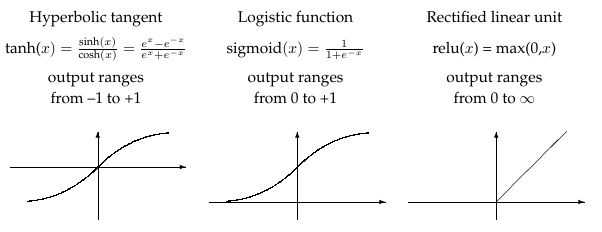
\includegraphics[width=0.9\textwidth]{activation_function.png}
\end{figure} 

A perceptron is the basic building blocks of neural network computation. Note that the output of a perceptron can be the input of another perceptron. 
In this manner, the perceptron can be interconnected to one and other, yielding complex networks. 

The following figure depicts a neural network with an additional layer between the input and output nodes:

\begin{figure}[h!]
\caption{A neural network with a hidden layer}
\centering
\begin{tikzpicture}[
plain/.style={
  draw=none,
  fill=none,
  },
net/.style={
  matrix of nodes,
  nodes={
    draw,
    circle,
    inner sep=10pt
    },
  nodes in empty cells,
  column sep=2cm,
  row sep=-9pt
  },
>=latex
]
\matrix[net] (mat)
{
|[plain]| \parbox{1.3cm}{\centering Input\\layer} & |[plain]| \parbox{1.3cm}{\centering Hidden\\layer} & |[plain]| \parbox{1.3cm}{\centering Output\\layer} \\
& |[plain]| \\
|[plain]| & \\
& |[plain]| \\
  |[plain]| & |[plain]| \\
& & \\
  |[plain]| & |[plain]| \\
& |[plain]| \\
  |[plain]| & \\
& |[plain]| \\    };
\foreach \ai [count=\mi ]in {2,4,...,10}
  \draw[<-] (mat-\ai-1) -- node[above] {Input \mi} +(-2cm,0);
\foreach \ai in {2,4,...,10}
{\foreach \aii in {3,6,9}
  \draw[->] (mat-\ai-1) -- (mat-\aii-2);
}
\foreach \ai in {3,6,9}
  \draw[->] (mat-\ai-2) -- (mat-6-3);
\draw[->] (mat-6-3) -- node[above] {Ouput} +(2cm,0);
\end{tikzpicture}

\rule{0in}{1.2em}$^\dag$\scriptsize For clarity, I don't show the bias nodes here.\\

\end{figure}    

This middle layer is called hidden layer. However, they are not really hidden; actually all the numerical values of each neuron in the hidden layer are all visible, but it is really hard to come up with a sensible interpretation on these numbers.  
When there are more than one hidden layers, the neural net is called deep neural net. However, the building blocks are still a simple perceptron. So, actually neural networks are simple and elegant computation operation\footnote{It seems to me that linking the perceptron is just like the simple Merge operation in the Minimalist Program.}; 
however, they extremely powerful. They are Turing-Complete machines \citep{siegelmann1991turing, graves2014neural}. \citet{siegelmann2003neural, siegelmann2012neural} even argues that neural networks are computations beyond the Turing limit. 



%\newpage
\subsection{Recurrent Neural Network}

Before we start to describe how a neural machine accomplishes the translation task, it is necessary to introduce a specific type of neural networks: Recurrent neural networks. 

Recall that the output of a perceptron can be the input of another perceptron. A interesting manipulation is to let the perceptron connect back to itself. With this manipulation, we have the Recurrent Neural Networks. As shown in the following figures, the hidden node is connected back to itself at each time step. As such, at each time step, there are two input sources of the hidden node: 1) the information from the past hidden node, and 2) the information from a new input node.       

\begin{figure}[h]
\caption{A recurrent neural network with a hidden layer. The hidden neuron ($h$) is connected to itself.}
\label{fig:rnn1}
\centering
\begin{tikzpicture}

  \node[neuron] (ht1) {$h$};
  \node[io,above=2em of ht1]  (yt1) {$y$};
  \node[io,below=2em of ht1]  (xt1) {$x$};
  \draw[conn] (ht1) -- (yt1);
  \draw[conn] (xt1) -- (ht1);
  \draw[thick,->,shorten >=1pt] (ht1.east) to [out=500,in=200,loop,looseness=4.8] (ht1.west);

\end{tikzpicture}
\end{figure}

\begin{figure}
\caption{A recurrent neural network with a hidden layer (unfolded depiction). This figure depicts exactly the same structure in figure \ref{fig:rnn1}, the hidden neuron $h_{t}$ is linked to its past $h_{t-1}$ and its future $h_{t+1}$. Here $t$ labels time step.}
\centering
\begin{tikzpicture}
\centering
  \node[neuron] (ht0)         {$h_{t-1}$};
  \node[io,above=2em of ht0] (yt)   {$y_{t-1}$};
  \node[io,below=2em of ht0] (xt)   {$x_{t-1}$};
  \draw[conn] (ht0) -- (yt);
  \draw[conn] (xt) -- (ht0);
  \node [left=of ht0] {\ldots};

  \node[neuron, right=of ht0] (ht1) {$h_{t}$};
  \node[io,above=2em of ht1]  (yt1) {$y_t$};
  \node[io,below=2em of ht1]  (xt1) {$x_t$};
  \draw[conn] (ht1) -- (yt1);
  \draw[conn] (xt1) -- (ht1);
  \draw [->] (ht0) -- (ht1);

  \node[neuron, right=of ht1] (ht2) {$h_{t+1}$};
  \node[io,above=2em of ht2]  (yt2) {$y_{t+1}$};
  \node[io,below=2em of ht2]  (xt2) {$x_{t+1}$};
  \draw[conn] (ht2) -- (yt2);
  \draw[conn] (xt2) -- (ht2);
  \draw [->] (ht1) -- (ht2);

  \node [right=of ht2] {\ldots};
\end{tikzpicture}
\end{figure}
\newpage
Is this manipulation useful? And if yes, why? It turns out Recurrent Neural Networks are really useful when we are interested in modeling a sequencing phenomenon and we believe that a fraction of the sequence will have an effect on the next coming fraction. The looping configuration opens the door to the history of the hidden neuron, and leads it to its future. 

Recurrent neural networks are widely used. Critically, the main theme of the dissertation, Neural Net Machine Translation, is also implemented with it. The coming section provides an overview of how neural networks translate languages. 

%\newpage
\section{Introduction to Neural Net Machine Translation}

My 3-year old daughter, Trina, is growing up in Tucson, Arizona, The languages that she encounters are English, Spanish and Mandarin Chinese, and thus she picks up English and Mandarin, and some Spanish. She is able to count the quantity of objects in the three languages. When I told her \textbf{in  Mandarin} that `we can bring two candies for Alice' on the way to her preschool, and she was able to tell her best friend, Alice, in her preschool that she will give her one candy \textbf{in English} (not two because Trina has to save one candy for herself).        

It is certain that a multilingual person can access the meaning of a sequence of strings in a language when he or she hears it, and then produces another sequence of strings in another different language with the same meaning. Given that a human brain is a neural network machine and artificial neural networks is similar to human neural networks, it fits our intuition that artificial neural networks can translate languages, of course. Actually, this is roughly how a neural net machine translation is implemented. Consider the following figure from \citet{luong17GitHub}.

\begin{figure}[h]
\caption{Encoder-decoder architecture - example of a general approach for NMT. An encoder converts a source sentence into a "meaning" vector which is passed through a decoder to produce a translation. (figure from \citet{luong17GitHub})}
\centering

\includegraphics[width=0.9\textwidth]{encdec.jpg}
\end{figure} 

The figure outlines the heuristic of how neural networks computation may translate languages. When the neural net is fed with a source sentence, ``I am a student'', it will convert the sentence into a meaning representation or a thought vector. This is the encoding process. Based on this meaning representation, the machine then derives another sequence of words in the target language. This is the decoding process. Now we may take a close look of how the encoding and decoding process works. 

\subsection{Word Embedding}
The neural machine can only process numeral representations, so the first step is to convert words into numerical representations. Specifically each word will be represented as a vector. The central idea is to map each word onto a location in ``a meaning space'', and each vector is the geographical coordinates of the word. 
This process is called word embedding. The ideal word embedding system would have the properties that words with similar meanings will be neighbors in the meaning space. 
The most commonly used technique of building word embeddings is proposed in \citet{mikolov2013efficient, mikolov2013distributed}. Critically, this word embedding implementation follows the distributional semantics philosophy: the meaning of a word is defined by its distribution in a corpus. So, to build a word embedding model all we need is a corpus. The training data for machine translation is a parallel corpus, which gives us two corpora: the source language corpus and target language corpus. So, the training data is sufficient for building word embedding models\footnote{It is also a common practice to build the word embedding separately using a bigger corpus when the parallel corpus is too small.}. The following figure depicts how it is like when the word embeddings are mapped to a 2D space.   

\begin{figure}
\caption{Word Embeddings (figure from \citet{roweis2000nonlinear})}
\centering
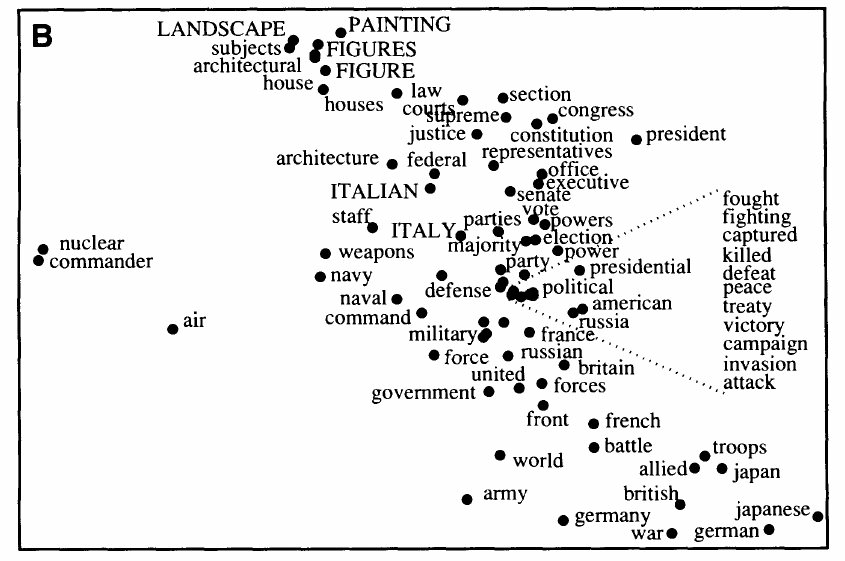
\includegraphics[width=0.9\textwidth]{word_emb.png}
\end{figure} 


\subsection{Encoding and Decoding}

A simple preprocessing on the data is to add tags that marks the boundaries of the sentences. Each word in the source sentence is sent to recurrent network machine incrementally. 
Note the looping configuration of recurrent neural networks makes it possible for the machine to accumulate the information of all the words. When the tag that marks the end of the source sentence is fed into the machine, the encoding process is completed, and the value of the hidden neurons at this time is the meaning representation of the source sentence.  

Given the meaning representation, now the machine starts to decode. At each time step, it emits a word in the target language. The emitted word in the target language is copied and served as input in the next time step of decoding. So that the output sentence can have the context information of the previous word; this trick ensures the fluency of the output sentence. 

Consider the following figure from \citet{luong17GitHub} for a concrete example of how the encoding-decoding process works.  

\begin{figure}[h]
\caption{Neural machine translation (figure from \citet{luong17GitHub}).}
\centering
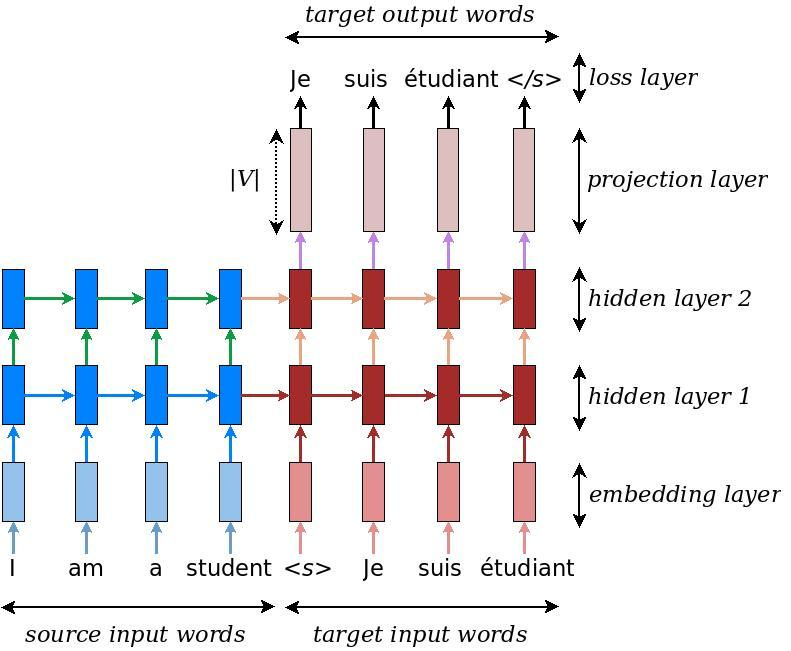
\includegraphics[width=0.9\textwidth]{seq2seq.jpg}
\end{figure} 

In the current example, we are trying to translate a source sentence ``I am a student'' into a target sentence ``Je suis \'{e}tudiant''. Here, ``<s>'' marks the end of the source sentences and the starting point of the decoding process. 
So, at the time step of  ``<s>'', the vector in the hidden neurons is the meaning representation. In the decoding process, the first emitted word is ``Je''. Note that ``Je'' is sent back as the input in the next time step, when ``suis'' is emitted. Now we may pay attention to what the given information is when the machine is emitting ``suis''. Specifically, the given information is: 1) thought vectors plus ``je'' in the hidden layers, and 2) ``je'' from the input node. When the machine emitted the tag, ``</s>'', the decoding process is completed. 

This section covers the basic structure of a neural machine translation system proposed in \citet{cho2014properties, cho2014learning}.  


\subsection{Adding Attention Mechanism}

The meaning vector is the accumulated information of all the bits in the source sentence. The decoding process needs to sort out all the bits from the mixed information in the meaning vector. Actually, this is a lot to ask. The task is like to figure out what ingredients are from a pot of hot and sour soup by tasting the soup. To facilitate the sorting task of the decoding processing, \citet{bahdanau2014neural} and \citet{luong2015effective} propose methods to direct the decoder's attention to the relevant bits in the source sentence. Take the soup analogy again. With the attention mechanism, to guess what the ingredient is, the given information is now the taste of vinegar, in addition to the taste of the mixed-up soup in this time step. So that the chance of getting the right answer (i.e. vinegar) is much higher. And in the next time step, in addition to the taste of the mixed-up soup, one is also given the taste of pepper, and so on.   

The following figure from \citet{luong17GitHub} nicely depicts how the attention mechanism works. 

\begin{figure}[h]
\caption{Attention mechanism - example of an attention-based NMT system as described in \citet{luong2015effective} (figure from \citet{luong17GitHub})}
\centering
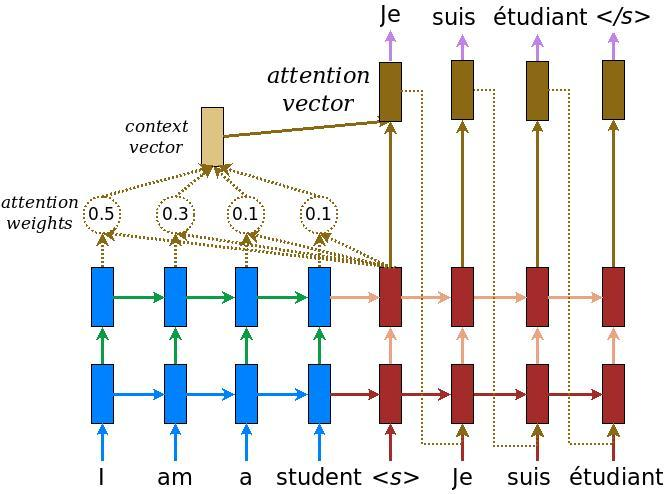
\includegraphics[width=0.9\textwidth]{attention_mechanism.jpg}
\end{figure} 

In the figure, the task is to translate a source sentence ``I am a student'' into a target sentence ``Je suis \'{e}tudiant''.
The encoding process is the same, but in the decoding process additional information is also provide. In the current example, when the decoder emits the word ``je'', it is given the meaning vector, and additionally the attention mechanism also gives the decoder 50\% of the information of ``I'', 30\% of the information of ``am'', 10\% of the information of ``a'', and 10\% of the information of ``student''. In this manner, the machine's attention is directed to ``I'' when the supposed emitted word is ``Je''. The attention mechanism is very similar to alignment; in the current example, ``Je'' is 50\% aligned to ``I'', 30\% aligned to ``am'', 10\% aligned to ``a'', and 10\% aligned to ``student''. 

\subsection{Summary of Neural Net Machine Translation: interlingua plus string alignment}

The state-of-the-art neural network machine translation is the combination of the encoding-decoding algorithm and the attention algorithm. The meaning vector in the encoding-decoding algorithm actually can be viewed as the holy grail in translation, the interlingua representation. The attention algorithm is a reminiscence of the string alignment approach used in statistical machine translation. So, neural net machine translation is actually a combination of interlingua  translation approach and string alignment approach.   


\section{A Quick Historical Overview of Machine Translation and Conclusion}

Machine Translation is to automate the process of translating one natural language to another using computers. The first peak of the developments of Machine Translation started in the 1940s but terminated in 1966. During this period of time, with the advent of the first computers, researchers held high expectations in Machine Translation and lots of resources are shifted into this area. 
ubHowever, in 1966 a report of the Automatic Language Processing Advisory Committee \citep{pierce1966language} terminated this `machine translation rush' as it revealed that too many funds and resources were shifted to Machine Translation without yielding proportional scientific developments. In 1990s, with the advent of Statistical Machine Translation approach developed at IBM, the Machine Translation came back as one of popular scientific areas. Now with the advent of the technique of Artificial Neural Net Machine Learning and other natural language processing techniques, Machine Translation is one of the most dynamic research areas.    
\chapter{Building Translation Systems using Interlinear Glossed Text: First Attempt}
\label{chap:cake}


\section{Introduction}
The Innovation is to incorporate the gloss information of Interlinear Glossed Text data into machine translation.

In supervised machine learning models, two factors effect the performance of the trained systems \citep{kotsiantis2007supervised}: a.) the quality of the training data and b.) the choice of the features. The properties of the gloss data as described in chapter \ref{chap:gloss} make it a better training data than natural language data (Scottish Gaelic in the current case) for the following reasons. First, glosses are more purified than natural language words. The most ideal meaning representation system should be built with one-meaning-to-one-representation mappings; in other words, a meaning is mapped to one and only one representation. Natural languages fail to do so, given that synonyms and ambiguous words/phrases are ubiquitous in natural languages. Glosses provide this one-to-one mapping. Second, the gloss data provides hierarchical (non-linear) syntactic parsing information. To determine what the gloss of a word is, linguists have to look for hierarchical (non-linear) context information. See chapter \ref{chap:gloss} for the discussion on the golden properties of glosses.  

Therefore, theoretically incorporation of the gloss data should improve the translation systems. Specifically, I propose the following hypothesis:
\begin{exe} 
\ex \label{gloss_helps_hypothesis}\textbf{Gloss-help hypothesis: the translation systems trained with the gloss data incorporated should outperform the systems trained with only Gaelic and English sentences pairs (i.e. without gloss data).}

The hypothesis can have two versions, strong and weak:
	\begin{xlist}
	\ex \label{strong_hy} Strong version: Gloss may replace the source natural language totally, and the system outperforms the system trained with source natural language to target language sentence pairs (i.e. the baseline systems).  
	\ex \label{weak_hy} Weak version: Gloss only increases the performance of the baseline systems, but cannot replace the source language.
	\end{xlist}
\end{exe}

The experiments in the current chapter will reveal that replacing Gaelic words with glosses doesn't boost up the performance of the translation systems. Thus, the strong version (replacing-Gaelic-with gloss) of the Gloss-help hypothesis is not empirically supported. 

This chapter describes the experiments conducted to test the strong version of the Gloss-help hypothesis.
The rest of the chapter is organized as follows: Section \ref{relate_work} describes related works in the literature, Section \ref{sec:experimet_setting} describes the constant parameter settings across all the experiments and the corpus used in the experiments, Section \ref{gd_to_gl_to_en} tests the hypothesis in (\ref{strong_hy}), Section \ref{section:cake1_Discussion} discusses the results and conclude this chapter.
%%%%%%%%%%%%%%%%%%%%%%%%%%%%%%%%%%%%%%%%%%%%%%%%%%%%%%%%%%%%%%%%%%%%%%%%%%%%%%%%%%%%%%%%%
\section{Related Work}\label{relate_work}
Attempts to improve machine translation systems by incorporating explicit linguistic information are reported in the literature. Syntax information is known to be effective in improving statistical machine translation (SMT). The efforts of using syntax information even derive a special type of SMT, termed as syntax-based SMT \citep{williams2016syntax}. The same trend is also found in neural net machine translation. For example, \citet{sennrich2016linguistic} exploit the information of lemmas, part of speech tags, morphology of words, and dependency parses of sentences to improve MT systems. \citet{ccg_target_seq} incorporate the Categorial grammar parse tags of the target sequences.

%%%%%%%%%%%%%%%%%%%%%%%%%%%%%%%%%%%%%5

\section{Technical Settings of the Machine Translation Experiments and Experimental Data of Scottish Gaelic Interlinear Glossed Text Corpus}\label{sec:experimet_setting}

\subsection{Technical Settings}
The experiments are conducted by using OpenNMT \citep{2017opennmt}, which implements the state-of-the-art neural net machine translation algorithms \citep{cho2014properties, cho2014learning, bahdanau2014neural}.
The following default hyper-parameter settings of OpenNMT\footnote{See their documentation for the complete default hyper-parameter settings: \url{http://opennmt.net/OpenNMT-py/}.} are used across all models so that the only independent variable is the type of the training data:
	\begin{itemize}
	\item Word vector size: 500\\
	In neural net machine translation, a word is represented as a vector. This hyper-parameter means that we are going to use vectors with 500 dimensions to represent words.
	\item Type of recurrent cell: Long Short Term Memory\\
	Long Short Term Memory recurrent neural net is a type of neural net that is suitable for sequence to sequence tasks.  
	\item Number of recurrent layers of the encoder and decoder: 2\\
	This hyper-parameter specifies that we are going to have two recurrent layers of the encoder and decoder. 
	\item Number of epochs: 13\\
	The training process of a neural net machine translation systems is done epoch by epoch. Each epoch is an iteration of training. Here 13 means that we are going to have 13 iterations of training and thus have 13 epochs. 
	\item Size of mini-batches: 64\\
	Training a neural net is to let the weights of the connections between the neurons fit the training samples. Theoretically, we may ask the neural net to adjust the weights according all the samples all together at one time. However, in practice, this is not memory efficient, and will cause errors in the process of optimizing the weight parameters. So, instead, the samples are split into smaller mini-batches, and the neural net just updates its weights to fit the samples in a mini-batch at one time. This hyper-parameter specifies the size of a mini-batch. Actually finding the right mini-batch size is not a trivial but an important question in Deep Learning. See \citet{DBLP:journals/corr/KeskarMNST16} and \citet{DBLP:journals/corr/abs-1711-00489} for the experiments and discussions on the effects of the size of mini-batches. 
	\end{itemize}

The settings of the hyper-parameters do have effects on the performances of the trained models.
A common practice to find the optimal settings of the hyper-parameters is to hold out a subset of the training dataset as the developing dataset, then test the models on the developing data to see what settings are optimal, then merge the developing dataset and training dataset as a new training set, and then train on this new training set using the found optimal hyper-parameters.

However, given that finding the optimal settings of the hyper-parameters is not relevant to our research and causes unnecessary complications, the process of optimizing the settings of the hyper-parameters is not implemented, and I simply adopt OpenNMT's default settings. The employed settings of the hyper-parameters should be viewed as arbitrarily chosen, and there are room to tune the models for better performance. Critically, these settings are viewed as constants, so that we can focus on the effects of different treatments on the source sequences in the translation experiments.  We will leave the question of what hyper-parameters are optimal for our data for future research.

\subsection{Experimental Data: a corpus of Scottish Gaelic Interlinear Glossed Texts}

We use the same Scottish Gaelic Interlinear Glossed Text corpus \citep{gaelic_igt} for all the experiments in chapter \ref{chap:cake} and chapter \ref{chap:cake2}. 
This corpus has 8,367 Gaelic sentences, and in term of words, it has 52,778 Gaelic words/glosses. The data of the corpus is from two different sources: linguistics fieldwork and data elicitation.

%The data and the scripts are accessible on GitHub\footnote{\url{https://github.com/lucien0410/Scottish_Gaelic}}, so that the results can be reproduced.  

\section{Gloss Representation Solely Does NOT Outperform Gaelic Sentences} \label{gd_to_gl_to_en}
This section tests the strong version of Gloss-help hypothesis in (\ref{strong_hy}).
Given the assumption that gloss may be better than any natural language in terms of representing meanings, it is expected that for neural net machine translation systems it is easier to learn how to translate from the glosses of Scottish Gaelic to English than to learn how to translate from Scottish Gaelic to English. However, the results show that there is no significant difference between the two types of data (i.e. GLOSS $\rightarrow$ English and Gaelic $\rightarrow$ English).

\subsection{Procedure of the Experiments}
I use repeated random sub-sampling validation to compare the performances of the two types of models.

Totally we have 8,388 indexed 3-tuples of a Gaelic sentence, a gloss line and an English translation. Each line in the interlinear glossed text example below is an argument of a 3-tuple sample.

\begin{exe} 
\ex \gll    Tha a athair nas sine na a mh\`athair.\\ 
           be.pres 3sm.poss father comp old.cmpr comp 3sm.poss mother
\\ 
   \glt    `His father is older than his mother.' 
\end{exe}

The 3-tuple representation of the above example is:
\begin{exe}
\ex <``Tha a athair nas sine na a mh\`athair'', ``be.pres 3sm.poss father comp old.cmpr comp 3sm.poss mother'', ``His father is older than his mother''>
\end{exe}

First, the samples (i.e. the 3-tuples) are randomly split into three datasets: training set (N=6,388), validation set (N=1,000), and test set (N=1,000)\footnote{Here the random sampling process is achieved by using the \begin{myfont}random.sample(population, k)\end{myfont} function in the standard library of python.}.

\begin{exe}
\ex Definitions of datasets:\\
	Let:
	\begin{xlist}
	\ex 	Index\textsubscript{Train}, Index\textsubscript{Validation}, and Index\textsubscript{Test} be sets of random indexes from 0 to 8,387.
   \ex		Index\textsubscript{Train} $\cap$ Index\textsubscript{Validation} $\cap$ Index\textsubscript{Test} = $\emptyset$
   \ex 	|Index\textsubscript{Train}| = 6,388; |Index\textsubscript{Validation}| = 1,000; |Index\textsubscript{Test}| = 1,000.
   \end{xlist}
\end{exe}
The step above just randomly splits the indexes of the 3-tuples into three distinct sets: Index\textsubscript{Train}, Index\textsubscript{Validation}, and Index\textsubscript{Test}. Based on the indexes, we generate the sets of samples. For each index, the 3-tuple is split into two pairs: <gloss, English>, <Gaelic, English>, so that later we can compare the different effects of gloss lines and Gaelic sentences. For each pair, the first item is the source sequence, and the second item is the target sequence. The systems learn how to map the source sequence to the target sequence.   

\begin{exe}
	\ex Gloss to English
		\begin{xlist}
		\ex \label{GLOSStoENTrain} GLOSStoEN\textsubscript{Train}   = $\{<gloss_i,En_i>  \mid i \in Index\textsubscript{Train} \}$ \\
		\ex \label{GLOSStoENVal} GLOSStoEN\textsubscript{Validation}   = $\{<gloss_i,En_i>  \mid i \in Index\textsubscript{Validation} \}$ \\
		\ex \label{GLOSStoENTest}GLOSStoEN\textsubscript{Test} = $\{<gloss_i,En_i>  \mid i \in Index\textsubscript{Test} \}$ \\
		\ex  Example: <``be.pres 3sm.poss father comp old.cmpr comp 3sm.poss mother'', ``His father is older than his mother.''>
		\end{xlist}

	
	\ex Gaelic to English
		\begin{xlist}
		\ex \label{GDtoENTrain} GDtoEN\textsubscript{Train}   = $\{<GD_i,En_i>  \mid i \in Index\textsubscript{Train} \}$ \\
		\ex \label{GDtoENVal} GDtoEN\textsubscript{Validation}   = $\{<GD_i,En_i>  \mid i \in Index\textsubscript{Validation} \}$ \\
		\ex \label{GDtoENTest} GDtoEN\textsubscript{Test}    = $\{<GD_i,En_i>  \mid i \in Index\textsubscript{Test} \}$ \\
		\ex Example: <``Tha a athair nas sine na a mh\`athair.'', ``His father is older than his mother.''>
		\end{xlist}
\end{exe}
The models are trained with the training set and validation set (i.e. the model learns how to map the source sequence to the target sequence). Both training set and validation set are known information for the models\footnote{Technically speaking, the validation set is part of the training data in terms of machine learning. The presence of the validation set is a special requirement of neural net machine learning, which uses the validation set to evaluate the convergence of the training.}. Specifically, the neural net system learns how to map gloss lines to English sentences from samples in (\ref{GLOSStoENTrain}) and (\ref{GLOSStoENVal}), and another neural net system learns how to map Gaelic sentences to English sentences from samples in (\ref{GDtoENTrain}) and (\ref{GDtoENVal}).

\begin{exe}
\ex Models:
	\begin{xlist}
	\ex \label{ModelGlossToEN} Model\textsubscript{GLOSStoEN} = Model trained with GLOSStoEN\textsubscript{Train} in (\ref{GLOSStoENTrain}) and GLOSStoEN\textsubscript{Validation} in (\ref{GLOSStoENVal})
	\ex \label{ModelGDToEN}Model\textsubscript{GDtoEN} = Model trained with GDtoEN\textsubscript{Train} in (\ref{GDtoENTrain}) and GDtoEN\textsubscript{Validation} in (\ref{GDtoENVal})
	\end{xlist}	
\end{exe}
The two trained models (gloss-to-English and Gaelic-to-English) then take the right source sequences of the test sets (i.e. glossing lines and Gaelic sentences for Model\textsubscript{GLOSStoEN} and Model\textsubscript{GDoEN} respectively) as inputs and then generate the predicted target sequences (i.e. English sentences).

\begin{exe}
\ex Predictions:
	\begin{xlist}
	\ex Predictions\textsubscript{GLOSStoEN} = A list of English sequences that Model\textsubscript{GLOSStoEN} maps to from the gloss sequences in (\ref{GLOSStoENTest})
	\ex Predictions\textsubscript{GDtoEN} = A list of English sequences that Model\textsubscript{GDtoEN} maps to from the Gaelic sentences in (\ref{GDtoENTest})
	\end{xlist}	
\end{exe}

To evaluate the model, the predicted target sequences are checked against the target sequences of the test set (i.e. the gold standard/human-translated English sentences).
Specifically, the BLEU (bilingual evaluation understudy)\footnote{There are other automatic machine translation evaluation algorithms available, such as translation edit rate \citep{Snover06astudy} and Damerau-Levenshtein edit distance \citep{damerau1964technique, levenshtein1966binary}. BLEU is chosen for the current experiments because it is the most widely used evaluation algorithm, and the correlation between the BLUE score evaluation and human judgment evaluation is also well-acknowledged.} score metric \citep{bleu} of each prediction is calculated using the \begin{myfont}multi-bleu.perl\end{myfont}\footnote{The script can be downloaded from: \url{https://github.com/moses-smt/mosesdecoder/blob/master/scripts/generic/multi-bleu.perl}}
script, a public implementation of Moses \citep{moses}. 


The BLEU assumes that a sentence is a bag of n-grams (n is from 1 to 4). It measures how different the two bags of n-grams (the predicted sentence and the gold standard sentence) are. A bag of words means that the order is not important, and the difference is measured by modified precision. For concreteness, consider the following toy examples:

\begin{exe}
\ex 
	\begin{xlist}
	\ex \label{gold1} Gold reference: `one two three four five'
	\ex \label{can1} predicted sentence 1: `one one two two two'
	\ex \label{can2} predicted sentence 2: `two two two one one'
	\end{xlist}
\end{exe}

For simplicity, let's consider unigram precision first. With the bag of words assumption, (\ref{can1}) and (\ref{can2}) are identical in terms of unigram because they have the same set\footnote{Here set does not mean the mathematical set but just unordered list.} of unigrams:   

\begin{exe}
\ex 
	\begin{xlist}
	\ex predicted sentence 1: `one one two two two' =\\
	 \{`one',`one',`two',`two',`two'\}  =\\
	 \{`two',`two', `two', `one', `one'\} =\\
	  predicted sentence 2: `two two two one one'
	\end{xlist}
\end{exe}

The unigram bag of word format of the gold-standard of our example is:

\begin{exe}
\ex gold-standard unigram bag of words
	\begin{xlist}
	\ex \{`one',`two',`three',`four',`five'\}
	\end{xlist}
\end{exe}

Now to calculate of the proportional similarity between the predicted bag of words and the gold-standard bags of words, BLEU uses `modified precision rate'. The technical meaning of `precision' is whether the predicted items are actually present in the gold-standard. Now the size of the bag of unigrams of the candidate is 5, the denominator of the precision rate is 5, and the denominator is how many items in the candidate set are present in the gold-standard. In the current example, \textit{one} and \textit{two} are both present in the gold-standard, so the denominator of (\ref{can1}) or (\ref{can2}) is 5. 
Now we have a wrongly inflated rate, 5 out of 5, 100$\%$ matched, meaning (\ref{can1}) or (\ref{can2}) is 100$\%$ similar to the gold-standard. 
To counter the effect of this inflation, BLEU uses `modified' precision rate. 
When the item in the gold-standard is matched, it is crossed-out, and invisible to the predicted bag of words\footnote{This is very similar to the feature checking mechanism in the Minimalist Program: one interpretable feature normally can only check out one uninterpretable feature.}. 
With this modified precision measurement, the two \textit{one}s only get one score and the three \textit{two}s only get one score. Now the modified precision rate is 2 out of 5, instead of 5 out of 5. 

In terms of bigrams, the same examples will be:

\begin{exe}
\ex 
	\begin{xlist}
	\ex \label{bi_gold1} Gold reference: \{`one\_two',  `two\_three', `three\_four', `four\_five'\}
	\ex \label{bi_can1} predicted sentence 1: \{`one\_one',  `one\_two', `two\_two', `two\_two'\}
	\ex \label{bi_can2} predicted sentence 2: \{`two\_two', `two\_two', `two\_one', `one\_one'\}
	\end{xlist}
\end{exe}

The denominator of the precision rate is 4 because the length of the predicted bag of words is 4; predicted sentence 1 in (\ref{bi_can1}) get 1 score because `one\_two' is matched, yielding a rate of 1 out of 4, while for predicted sentence 2 in (\ref{bi_can2}) no bigram is matched, yielding a rate of 0 out of 4. 

A loose end of the current measurement is that it will wrongly give a shorter predicted sentence a higher precision rate because the shorter the smaller the denominator is. To counter this, the final version of BLUE penalizes short predicted sentence by multiplying the ratio between the length of the predicted sequence and the length of the gold-standard sentence. For N from 1 to 4, each N-gram comparison yields a BLEU score; the multi-BLEU score is just the combination of the 4 BLEU scores (unigram to four-gram). 

Put all together, a concise way of describing the calculation of BLUE is the following equation.  

\maths{\begin{equation} 
\text{\sc bleu} = \min \left( 1,\frac{\text{\em output-length}}{\text{\em reference-length}} \right) \; \big( \prod_{i=1}^4 \text{\em precision}_i \big)^\frac{1}{4}
\end{equation}}

For a little bit more complicated example of calculating the multi-bleu score, consider the following example in figure \ref{bleu_koeh} from \citet[p. 226-227]{koehn2009statistical}.

\begin{figure}[t] \label{bleu_koeh}
\caption{The BLEU score is based on n-gram matches with the reference translation \citep[p. 226-227]{koehn2009statistical}} \label{bleu_koeh}
\begin{center}
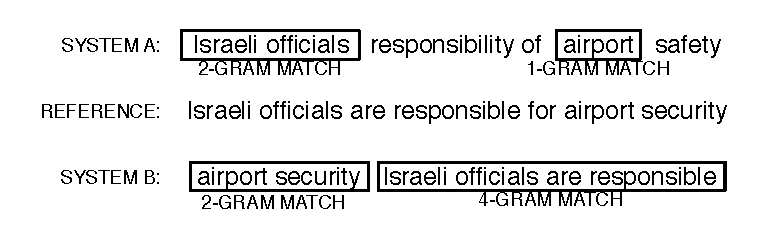
\includegraphics[scale=1.5]{bleu-example.pdf}
\begin{tabular}{c|c|c}
{\bf Metric} & \bf System A & \bf System B \\ \hline
precision (1gram) & 3/6 & 6/6 \\ \hline
precision (2gram) & 1/5 & 4/5 \\ \hline
precision (3gram) & 0/4 & 2/4 \\ \hline
precision (4gram) & 0/3 & 1/3  \\ \hline
brevity penalty   & 6/7 & 6/7  \\ \hline 
{\sc bleu} &  0\% & 52\%  \\ \hline
\end{tabular}
\end{center}
\end{figure}


In short, the BLEU score calculation is an automatic evaluation of how similar two copora are. In the current experiments we are comparing the predicted target sequences with the gold standard. The BLEU score of 100 means the two copora are identical, and the BLEU score of 0 means the two copora are completely distinct from each other.

\begin{exe}
\ex Gold-Standard = English sentences in (\ref{GLOSStoENTest}) = English sentences in (\ref{GDtoENTest})
\end{exe}
Note that the gold-standard is the same because they are the same English sentences in the 3-tuples samples. Then the two sets of predicted English sentences are evaluated, yielding two BLEU scores.  

\begin{exe}
\ex Scores: \\
 \begin{xlist}
	\ex Score\textsubscript{GLOSStoEN} = BLEU(Gold-Standard, Predictions\textsubscript{GLOSStoEN}) \\
	\ex Score\textsubscript{GDtoEN} = BLEU(Gold-Standard, Predictions\textsubscript{GDtoEN}) \\
 \end{xlist}
\end{exe}
This procedure of splitting the data into three sub-sets, training the models, and evaluating the models is executed ten times.

\subsection{Result} \label{gdglen_results}
After ten rounds of repeated random sub-sampling validation, ten pairs of scores of the two models are generated, as shown in the following table.
% !Rnw root = cake_chapter.Rnw
% latex table generated in R 3.4.4 by xtable 1.8-2 package
% Tue May  1 00:04:46 2018
\begin{table}[ht]
\centering
\begin{tabular}{lcc}
  \hline
Round & Gaelic (Baseline) & GLOSS \\ 
  \hline
0 & 17.29 & 18.39 \\ 
  1 & 16.42 & 18.00 \\ 
  2 & 15.29 & 16.02 \\ 
  3 & 15.97 & 20.22 \\ 
  4 & 17.79 & 19.02 \\ 
  5 & 16.73 & 15.53 \\ 
  6 & 17.11 & 18.00 \\ 
  7 & 16.37 & 20.08 \\ 
  8 & 15.93 & 15.82 \\ 
  9 & 16.99 & 15.93 \\ 
   \hline
Mean & 16.59 & 17.70 \\ 
   \hline
\end{tabular}
\caption{BLEU scores of Model\textsubscript{GDtoEN} and Model\textsubscript{GLOSStoEn}} 
\label{Table:GLOSS}
\end{table}
The average score of the Models\textsubscript{GLOSStoEN} is only slightly higher than the average score of the Models\textsubscript{GDtoEN}.
Also, after doing a paired T-test, the difference between the two types of models is not attested
(M\textsubscript{GDToEn}=16.59, SD\textsubscript{GDToEn}=0.74; M\textsubscript{GLOSStoEN}=17.70, SD\textsubscript{GLOSStoEN}=1.78; t(9)=1.97, p=0.080)

\subsection{Summary}
The ultimate practical goal of the dissertation is to use glossing data to develop better machine translation systems. Here \textit{better} means to be better than a baseline system, which is the machine translation system trained with Gaelic-to-English translation samples. The models in (\ref{ModelGDToEN}) are the baseline systems, and their scores are in the Gaelic column of table (\ref{Table:GLOSS}). These are the target scores that we aim to outperform. The experiment above is the first attempt to improve the scores by using the \textit{gloss treatment}, in which the Gaelic sentences are replaced with gloss lines.  However, the result shows that this \textit{gloss treatment} is not effective as the scores of the gloss models are not statistically higher than the baseline Gaelic-to-English models. 

\section{Discussion and Conclusion}\label{section:cake1_Discussion}
It is assumed that the performances of the machine translation systems are correlated with the quality of the representation of meanings in the source sequences. Better representations of meanings yield better machine translation systems. Given the results in (\ref{gdglen_results}) that the gloss models are not better than the Gaelic models, it is concluded that glosses and natural languages are equally good in terms of representing meanings. The strong version of the Gloss-help hypothesis does not hold.

There are several remarks that need to be addressed for the current result. 

First, the result falsifies the point of view about glosses in chapter (\ref{chap:gloss}) that the gloss line is a golden semantic representation hand-crafted by linguists.
It turns that this artificial language, the gloss lines, is only marginal better than Gaelic, as the mean BLEU score of the gloss treatment is slightly higher than that of the baseline systems. This can be viewed as an evidence of language evolution.
The written form of a natural language is actually already optimized for representing semantics to the same degree of gloss line representations.

Second, if we want to actually apply the gloss treatment to translate a Gaelic sentence to English, we encounter an immediate problem. The actual source sequence is a Gaelic sentence, while the required source sequence for the gloss treatment is a gloss line. The auto-glosser described in chapter (\ref{chap:gloss}) may convert the Gaelic sentence to a gloss line, but the conversion is not perfect at all. Given this, even if the gloss treatment should work, it is not practical unless we may convert Gaelic sentence to gloss line perfectly.      

We may now combine Gaelic and Gloss sentences as the training data to test the weak version of the Gloss-help hypothesis. The experiments and results are reported in the next chapter.
%%%%%%%%%%%%%%%%%%%%%%%%%%%%%%%%%%%%%%%%%%%%%%%%%%%%%%%%%%%%%%%%%%%%%%%%%%%%%%%%%%%%%%%%%%%
\chapter{Combining Gaelic Words with Glosses}\label{chap:cake2}
\section{Introduction}
In the previous chapter, we attempt to build a system by using the \textit{gloss treatment} to outperform the baseline system. It turns out that solely using gloss line is not effective enough to improve the system. However, this result does not falsify the gloss-help hypothesis; instead, it indicates that combination of the gloss line data and the Gaelic sentence data is necessary. In other words, the questions now are: 
\begin{exe}
	\ex 
	\begin{xlist}
		\ex Does adding the gloss data into the Gaelic data will improve the translation system? 
		\ex If yes, what are the right ways of blending these two types of meaning representations together? 
	\end{xlist}	
\end{exe}

This section reports various ways of combining the gloss line data and the Gaelic sentence data, and the experiments and their results using these different treatments. Critically, a specific way of combining Gloss data and Gaelic date (termed as `\textit{Parallel-Partial}' treatment) boosts the performance significantly. The model trained with this specially arranged training data also significantly outperforms Google's Gaelic-to-English translation system.

In this section, I will first describe the most effective treatment, termed as `\textit{Parallel-Partial}' treatment, and the results. Next, I will report the experiments done with other relevant logical treatments (i.e. other ways of combining glossing data and Gaelic data). 

\subsection{The Underlying Heuristics}\label{heuristics}
At a high level, neural net sequence to sequence learning algorithm is learning how to map a high-dimension space to another high-dimension space. In the settings of machine translation, each dot in the high-dimension space is a meaning representation. Linking one dot to another dot is converting one representation of meaning to another, yielding the effect of translation. Given this heuristics, we may just feed the machine with all the available meaning mappings. Given the assumption that the gloss lines are linguistically guided representations of meaning, they are suitable training data for building machine translation systems. Specially, with the gloss data, we let the machine to learn the following mappings:

\begin{exe}
	\ex Mappings Learned in the ParaPart treatment
	\begin{xlist}
		\ex Gaelic sentences $\rightarrow$ English sentences
		\ex Gloss lines $\rightarrow$ English sentences
		\ex Gloss lines $\rightarrow$ Gaelic sentences
		\ex Gaelic words $\rightarrow$ Gloss items
	\end{xlist}	
\end{exe}    

\section{The `Parallel-Partial' Treatment Outperforms Any Other Treatments and the Baseline Significantly}

\subsection{Related work}
The Parallel-Partial treatment section may be viewed as a form of multi-task Sequence to Sequence Learning \citep{luong2015multi}. Specifically, the parallel part of the treatment is very similar to the data manipulation used in building multi-language translation systems \citep{google_zero_shot}.  

\subsection{Data Preprocessing Using the Parallel-Partial Treatment}
The Parallel-Partial treatment uses the training and validation data of the baseline system and that of the gloss treatment system.  
The training and validation data of the baseline system are pairs of a Gaelic sentence and a English sentence (see (\ref{GDtoENTrain}) and (\ref{GDtoENVal}) ), 
and the data of the gloss treatment are pairs of a gloss line and a English sentence (see (\ref{GLOSStoENTrain}) and (\ref{GLOSStoENVal}). 
These two groups of data are combined in a parallel manner in the current treatment. Now the sizes of training set and validation set are doubled. In the baseline system and the gloss treatment system, we have 6,388 samples in the training set and 1,000 samples in the validation set. The current treatment has 12,776 samples in the training set and 2,000 samples in the validation set. This is the \textit{parallel} part of the treatment. 

Additionally, I utilize the alignment property between the Gaelic word and the gloss to further build pairs of a Gaelic word and a gloss. These pairs are also included into the training set and validation set of the current treatment. This is the \textit{partial} part of the treatment.   

For concreteness, consider the following interlinear glossed text: 
\begin{exe}  
\ex \gll    Tha a athair nas sine na a mh\`athair.\\  
            be.pres 3sm.poss father comp old.cmpr comp 3sm.poss mother\\  
    \glt    `His father is older than his mother.'  
\end{exe}

With the interlinear glossed text, the parallel treatment will generate three pairs of samples:

\begin{exe}
	\ex\label{sample_para}
	\begin{xlist}
		\ex Gaelic to English: \\<``Tha a athair nas sine na a mh\`athair'', ``His father is older than his mother.''>
		\ex Gloss to English: \\<``be.pres 3sm.poss father comp old.cmpr comp 3sm.poss mother'', ``His father is older than his mother''>
		\ex Gloss to Gaelic: \\<``be.pres 3sm.poss father comp old.cmpr comp 3sm.poss mother'', ``Tha a athair nas sine na a mh\`athair''>
	\end{xlist}
\end{exe}

The partial treatment then generates pairs of a Gaelic word and a gloss token: 
\begin{exe}
	\ex\label{sample_partial}
	\begin{xlist}
		\ex <``Tha'', ``be.pres''>
		\ex <``a'', ``3sm.poss''>
		\ex <``athair'', ``father''>
		\ex <``nas'', ``comp''>
		\ex <``sine'', ``old.cmpr''>
		\ex <``na'', ``comp''>
		\ex <``a'', ``3sm.poss''>
		\ex <``mh\`athair'', ``mother''>
	\end{xlist}
\end{exe}

The samples in (\ref{sample_para}) and (\ref{sample_partial}) are the training data for this Parallel-Partial treatment. 

\subsection{Results of the Parallel-Partial Treatment}

Critically, the same technical settings and the same test sets in the previous experiments are used, and the same procedures are executed. The same split of the original IGTs is used, so as long as it is the same round, the training, validation and test are the same set of IGTs. The only difference is that now the training and validation IGT data are treated with the Parallel-Partial treatment. The results show that the Parallel-Partial treatment has a tremendous effect in improving the baseline system. 

% !Rnw root = cake_chapter.Rnw
% latex table generated in R 3.4.4 by xtable 1.8-2 package
% Tue May  1 00:04:47 2018
\begin{table}[ht]
\centering
\begin{tabular}{lcc}
  \hline
Round & Gaelic (Baseline) & ParaPart \\ 
  \hline
0 & 17.29 & 32.64 \\ 
  1 & 16.42 & 32.28 \\ 
  2 & 15.29 & 29.94 \\ 
  3 & 15.97 & 31.18 \\ 
  4 & 17.79 & 32.83 \\ 
  5 & 16.73 & 31.11 \\ 
  6 & 17.11 & 32.19 \\ 
  7 & 16.37 & 33.52 \\ 
  8 & 15.93 & 30.93 \\ 
  9 & 16.99 & 34.35 \\ 
   \hline
Mean & 16.59 & 32.10 \\ 
   \hline
\end{tabular}
\caption{BLEU scores of Model\textsubscript{GDtoEN} and Model\textsubscript{ParaParttoEn}} 
\label{Table:ParaPart}
\end{table}
The first and the second columns are BLUE scores of the baseline systems and the systems with the Parallel-Partial treatment respectively. The latter is significantly better than the former
(M\textsubscript{GDToEn}=16.59, SD\textsubscript{GDToEn}=0.74; M\textsubscript{ParaPart}=32.10, SD\textsubscript{ParaPart}=1.33; t(9)=48.95, p<0.01).
The comparison of the average BLUE scores of the groups of systems shows that the Parallel-Partial treatment improves the performance of the baseline system by 93 percent.
%(M\textsubscript{GDToEn}=16.59, SD\textsubscript{GDToEn}=0.74; M\textsubscript{ParaPart}=32.10, SD\textsubscript{ParaPart}=1.33,; t(9)=48.95, p<0.010.000).
\subsubsection{Discussion}
With the ParaPart treatment, the baseline systems are improved for more than 93 percent. This result suggests the validity of our heuristics in section \ref{heuristics} that gloss lines can be viewed as an artifical language, and provide strong evidence for the gloss-help hypothesis in (\ref{gloss_helps_hypothesis}).     


%%%%%%%%%%%%%%%%%%%%%%%%%%%%%%%%%%%%
\section{Other Possible Treatments}
This section reports other possible ways of blending the Gaelic sentences and gloss lines\footnote{There must be other possible and logical ways to blend in gloss that are beyond my imagination. It seems me to that by simply attempting to incorporate gloss information we open many other doors to the possible ways of improving machine translation systems. This is another merit of combining theoretical linguists to natural language processing.}.
However, all of these treatments are not as effective as the Parallel-Partial treatment. Again, the same procedure and the same test datasets are used across all the experiments. 


\subsection{The Parallel Treatment}\label{treatment:Para}
\subsubsection{Method of the Parallel Treatment}
The Parallel treatment is using the parallel part of the Parallel-Partial treatment without exploiting the alignment properties of gloss lines.
It is expected that this treatment will improve the baseline systems but will not be as effective as the Parallel-Partial treatment.

With this treatment, a chunk of interlinear glossed text is split into two pairs. For example, the chunk of interlinear glossed text in (\ref{igt}) becomes two samples in (\ref{sample_pair}): 
\begin{exe} 
\ex \label{igt}
	\gll    Tha a athair nas sine na a mh\`athair.\\  
            be.pres 3sm.poss father comp old.cmpr comp 3sm.poss mother \\
    \glt    `His father is older than his mother.'  
\end{exe}


\begin{exe} 
	\ex \label{sample_pair}
	\begin{xlist}
		\ex Gaelic to English: \\<``Tha a athair nas sine na a mh\`athair'', ``His father is older than his mother.''>
		\ex Gloss to English: \\<``be.pres 3sm.poss father comp old.cmpr comp 3sm.poss mother'', ``His father is older than his mother''>
	\end{xlist}
\end{exe}

\subsubsection{Results of the Parallel Treatment}\label{treatment:Para_result}
The experiments gave us the expected results. 
% !Rnw root = cake_chapter.Rnw
% latex table generated in R 3.4.4 by xtable 1.8-2 package
% Tue May  1 00:04:47 2018
\begin{table}[ht]
\centering
\begin{tabular}{lcc}
  \hline
Round & Gaelic (Baseline) & Para \\ 
  \hline
0 & 17.29 & 30.40 \\ 
  1 & 16.42 & 30.07 \\ 
  2 & 15.29 & 26.05 \\ 
  3 & 15.97 & 29.67 \\ 
  4 & 17.79 & 28.86 \\ 
  5 & 16.73 & 29.46 \\ 
  6 & 17.11 & 30.57 \\ 
  7 & 16.37 & 30.45 \\ 
  8 & 15.93 & 28.83 \\ 
  9 & 16.99 & 31.28 \\ 
   \hline
Mean & 16.59 & 29.56 \\ 
   \hline
\end{tabular}
\caption{BLEU scores of Model\textsubscript{GDtoEN} and Model\textsubscript{ParatoEn}} 
\label{Table:Para}
\end{table}The table in (\ref{Table:Para}) compares the performances of this treatment and the baseline. Critically, the Parallel treatment is effective in improving the baseline systems (M\textsubscript{GDToEn}=16.59, SD\textsubscript{GDToEn}=0.74; M\textsubscript{Para}=29.56, SD\textsubscript{Para}=1.46; t(9)=34.42, p < 0.01). 
% !Rnw root = cake_chapter.Rnw
%GDParaParaPart1_table.Rnw does NOT print out anything but just load the sexpr variables 
However, the best treatment (i.e. the Parallel-Partial treatment) is still far better than this Parallel treatment 
(M\textsubscript{Para}=29.56, SD\textsubscript{Para}=1.46; M\textsubscript{ParaPart}=32.10, SD\textsubscript{ParaPart}=1.33; t(9)=8.76, p < 0.01 ).
% !Rnw root = cake_chapter.Rnw
% latex table generated in R 3.4.4 by xtable 1.8-2 package
% Tue May  1 00:04:47 2018
\begin{table}[ht]
\centering
\begin{tabular}{lccc}
  \hline
Round & Gaelic (Baseline) & Para & ParaPart \\ 
  \hline
0 & 17.29 & 30.40 & 32.64 \\ 
  1 & 16.42 & 30.07 & 32.28 \\ 
  2 & 15.29 & 26.05 & 29.94 \\ 
  3 & 15.97 & 29.67 & 31.18 \\ 
  4 & 17.79 & 28.86 & 32.83 \\ 
  5 & 16.73 & 29.46 & 31.11 \\ 
  6 & 17.11 & 30.57 & 32.19 \\ 
  7 & 16.37 & 30.45 & 33.52 \\ 
  8 & 15.93 & 28.83 & 30.93 \\ 
  9 & 16.99 & 31.28 & 34.35 \\ 
   \hline
Mean & 16.59 & 29.56 & 32.10 \\ 
   \hline
\end{tabular}
\caption{BLEU scores of Model\textsubscript{GDtoEN}, Model\textsubscript{ParatoEN} and Model\textsubscript{ParaParttoEN} } 
\label{Table:Concating}
\end{table}
Critically, the comparison between the Parallel-Partial treatment and current Parallel-Only treatment shows the effectiveness of the word-gloss alignments. Our conjecture on the effectiveness is that with the pairs of a gloss item and a Gaelic word present in the training data, the burden of the attention algorithm \citep{bahdanau2014neural} is largely alleviated. In other words, instead of asking the attention algorithm to estimate what to attend to, we explicitly teach the machine the alignment between the Gaelic word and the corresponding gloss. 

%%%%%%%%%%%%%%%%%%%%%%%%%%%%%%%%%%%%%%%%%%%%%%%%%%%5
\subsection{Interleaving Gaelic Words and Gloss Items And Concating them}\label{treatment:InterleavingAndConCat}
\subsubsection{Method of the Interleaving Treatment}

Instead of putting the pairs of a Gaelic sentence and a English sentence and the pairs of a gloss line and a English sentence in a parallel manner,
we may just literally blend a Gaelic sentence and a gloss line by interleaving them\footnote{\citet{ccg_target_seq} incorporate the Categorial grammar parse tags into natural sentences by interleaving the tags and the words.}. Consider the following example:

\begin{exe} 
\ex 
	\begin{xlist}
	\ex \label{ex_interleave:in}
		\gll	 Tha a athair nas sine na a mh\`athair.\\  
     		     be.pres 3sm.poss father comp old.cmpr comp 3sm.poss mother \\
    	\glt    `His father is older than his mother.'  

    \ex \label{ex_interleave:out} <``Tha be.pres a 3sm.poss athair father nas comp sine old.cmpr na comp a 3sm.poss mh\`athair mother'', ``His father is older than his mother''>
    \end{xlist}
\end{exe}

Given the chuck of interlinear glossed text data in (\ref{ex_interleave:in}), the Interleaving treatment generates the sample in (\ref{ex_interleave:out}).  

This way of blending gloss lines and Gaelic sentences may add useful information into the training data; 
however, the downside of this method is to increase the length of the source sequence. In neural net machine learning, the longer the sequences are, the harder it is to preserve all the information (i.e. it is harder for the attention mechanism to pay attention to the right tokens). So, this treatment may not be effective. 


The results are given in the following table. 
% !Rnw root = cake_chapter.Rnw
% latex table generated in R 3.4.4 by xtable 1.8-2 package
% Tue May  1 00:04:47 2018
\begin{table}[ht]
\centering
\begin{tabular}{lcc}
  \hline
Round & Gaelic (Baseline) & interleavingGdGLOSS \\ 
  \hline
0 & 17.29 & 13.67 \\ 
  1 & 16.42 & 12.49 \\ 
  2 & 15.29 & 11.01 \\ 
  3 & 15.97 & 12.33 \\ 
  4 & 17.79 & 12.56 \\ 
  5 & 16.73 & 12.13 \\ 
  6 & 17.11 & 11.55 \\ 
  7 & 16.37 & 12.78 \\ 
  8 & 15.93 & 12.43 \\ 
  9 & 16.99 & 11.65 \\ 
   \hline
Mean & 16.59 & 12.26 \\ 
   \hline
\end{tabular}
\caption{BLEU scores of Model\textsubscript{GDtoEN} and Model\textsubscript{interleavingGdGLOSStoEn}} 
\label{Table:interleavingGdGLOSS}
\end{table}\newline
It turns out this treatment has a significant negative effect
(M\textsubscript{GDToEn}=16.59, SD\textsubscript{GDToEn}=0.74; M\textsubscript{interleavingGdGLOSS}=12.26, SD\textsubscript{interleavingGdGLOSS}=0.74,; t(9)=-17.06, p=0.000). This is not the right way of incorporating gloss line data. 

%%%%%%%%%%%%%%%%%%%%%%%%%%%%%%%%%%%%%%%%%%%%%%%%%%%%%%%%%%%%%
\subsubsection{Method of Concatenating Gaelic Words and Gloss Words }\label{treatment:Concating}
A quick and close amendment of the Interleaving approach is to concatenate the aligned Gaelic word and gloss item as a single token. Given the same chunk of interlinear glossed text data, this treatment generates the following sample:

\begin{exe} 
\ex 
	\begin{xlist}
	\ex 
		\gll	 Tha a athair nas sine na a mh\`athair.\\  
     		     be.pres 3sm.poss father comp old.cmpr comp 3sm.poss mother \\
    	\glt    `His father is older than his mother.'  

    \ex <``Tha\_be.pres a\_3sm.poss athair\_father nas\_comp sine\_old.cmpr na\_comp a\_3sm.poss mh\`athair\_mother'', ``His father is older than his mother''>
    \end{xlist}
\end{exe}

Concatenating words and glosses does solve the long sequence problem; however, it causes the sparse data problem. In this arrangement, the number of the types of tokens is increased; the number of tokens of each type is decreased. Thus, all the samples are put in a larger space. So, the treatment may not be effective either. 

\subsubsection{Results of Concating Gaelic Words and Gloss Words}
The performances of this treatment is given in the following table.
% !Rnw root = cake_chapter.Rnw
% latex table generated in R 3.4.4 by xtable 1.8-2 package
% Tue May  1 00:04:47 2018
\begin{table}[ht]
\centering
\begin{tabular}{lcc}
  \hline
Round & Gaelic (Baseline) & ConcatGLOSSGaelic \\ 
  \hline
0 & 17.29 & 15.42 \\ 
  1 & 16.42 & 14.31 \\ 
  2 & 15.29 & 15.38 \\ 
  3 & 15.97 & 14.18 \\ 
  4 & 17.79 & 18.63 \\ 
  5 & 16.73 & 14.89 \\ 
  6 & 17.11 & 15.16 \\ 
  7 & 16.37 & 15.20 \\ 
  8 & 15.93 & 15.50 \\ 
  9 & 16.99 & 15.72 \\ 
   \hline
Mean & 16.59 & 15.44 \\ 
   \hline
\end{tabular}
\caption{BLEU scores of Model\textsubscript{GDtoEN} and Model\textsubscript{ConcatGLOSSGaelictoEn} } 
\label{Table:Concating}
\end{table}\newline
The result shows that this treatment hurts the baseline systems instead of improving them (M\textsubscript{GDToEn}=16.59, SD\textsubscript{GDToEn}=0.74; M\textsubscript{ConcatGLOSSGaelic}=15.44, SD\textsubscript{ConcatGLOSSGaelic}=1.23,; t(9)=-3.64, p=0.010).

%%%%%%%%%%%%%%%%%%%%%%%%%%%%%%%%%%
\subsection{Hybrid: Gaelic or Gloss}
\subsubsection{Method of Hybrid}
The Hybrid treatment aims to reduce the potential lexical ambiguity. A Gaelic word may map to multiple glosses, and a glosses may map to multiple Gaelic words. Let's assume a toy example of a chunk of interlinear glossed text data (a one-word sentence): 

\begin{exe} 
\ex 
	\gll	 Gaelic\_word\\  
     		 Gloss\_item \\
    \glt    English translation  
\end{exe} 

Now we aim to build a single sample that is either <Gaelic\_word, English translation > or <Gloss\_item, English translation >. To decide, we need to know which one, the Gaelic word or the gloss item, is less ambiguous. 
The less ambiguous one is the winner. For example, if the Gaelic word is potentially mapped to 10 glosses and if the gloss item is potentially mapped 2 Gaelic words, then <Gloss\_item, English translation> is chosen; on the other hand, if the ambiguity situation is reverted, then <Gaelic\_word, English translation > is chosen. 
However, when the situation is tight (i.e. both the Gaelic word and gloss item are equally ambiguous), a default setting needs to be chosen. The choices of the default setting split this single treatment into two treatments: default as Gaelic or default as gloss.

The following is an example of the hybrid treatment:

\begin{exe}
\ex
	\gll tha nathairichean a'chuir an t-eagal orm\\
		 be.pres snake.vn put det fear on.1s\\
	\glt `Snakes frighten me' 
\end{exe} 

The length of the Gaelic sentence and the gloss line in the above IGT is 6. This means 6 ambiguity comparisons need to be made to decide which one, Gaelic word or gloss, should take the position. The final production of this hybrid treatment on the above IGT is shown as follows:

\begin{exe}
\ex <``be.pres nathairichean a'chuir det t-eagal on.1s'' ,``Snakes frighten me'' >
\end{exe} 

This treatment has the same potential downside as the concatenating treatment: sparsity. In this treatment, the size of the lexicon is the size of the lexicon of Gaelic word plus that of gloss, but what are really visible to the neural net is only about half size of the whole potential lexicon, because for each position it is either a Gaelic word or a gloss.

\subsubsection{Result of Hybrid}    
% !Rnw root = cake_chapter.Rnw
% latex table generated in R 3.4.4 by xtable 1.8-2 package
% Tue May  1 00:04:47 2018
\begin{table}[ht]
\centering
\begin{tabular}{lcc}
  \hline
Round & Gaelic (Baseline) & HybridDefaultAsGaelic \\ 
  \hline
0 & 17.29 & 9.44 \\ 
  1 & 16.42 & 9.07 \\ 
  2 & 15.29 & 7.69 \\ 
  3 & 15.97 & 9.12 \\ 
  4 & 17.79 & 9.08 \\ 
  5 & 16.73 & 10.45 \\ 
  6 & 17.11 & 8.62 \\ 
  7 & 16.37 & 10.00 \\ 
  8 & 15.93 & 10.52 \\ 
  9 & 16.99 & 8.46 \\ 
   \hline
Mean & 16.59 & 9.24 \\ 
   \hline
\end{tabular}
\caption{BLEU scores of Model\textsubscript{GDtoEN} and Model\textsubscript{HybridDefaultAsGaelictoEn}} 
\label{Table:HybridDefaultAsGaelic}
\end{table}When the default setting is the Gaelic word, the performances are significantly worse than the baseline systems
(M\textsubscript{GDToEn}=16.59, SD\textsubscript{GDToEn}=0.74; M\textsubscript{ReplacingGaelic}=9.24, SD\textsubscript{ReplacingGaelic}=0.89,; t(9)=-21.03, p < 0.01), 
as shown in table (\ref{Table:HybridDefaultAsGaelic}).

% !Rnw root = cake_chapter.Rnw
% latex table generated in R 3.4.4 by xtable 1.8-2 package
% Tue May  1 00:04:47 2018
\begin{table}[ht]
\centering
\begin{tabular}{lcc}
  \hline
Round & Gaelic (Baseline) & HybridDefaultAsGLOSS \\ 
  \hline
0 & 17.29 & 15.95 \\ 
  1 & 16.42 & 15.60 \\ 
  2 & 15.29 & 14.15 \\ 
  3 & 15.97 & 14.72 \\ 
  4 & 17.79 & 15.74 \\ 
  5 & 16.73 & 14.88 \\ 
  6 & 17.11 & 14.45 \\ 
  7 & 16.37 & 16.41 \\ 
  8 & 15.93 & 15.15 \\ 
  9 & 16.99 & 17.61 \\ 
   \hline
Mean & 16.59 & 15.47 \\ 
   \hline
\end{tabular}
\caption{BLEU scores of Model\textsubscript{GDtoEN} and Model\textsubscript{HybridDefaultAsGLOSS}} 
\label{Table:HybridDefaultAsGLOSS}
\end{table}When the default setting is the Gaelic word, the performances are sightly worse than than the baseline systems 
(M\textsubscript{GDToEn}=16.59, SD\textsubscript{GDToEn}=0.74; M\textsubscript{ReplacingGaelic}=15.47, SD\textsubscript{ReplacingGaelic}=1.03,; t(9)=-3.67, p < 0.01 ), as shown in table (\ref{Table:HybridDefaultAsGLOSS}).

The results show that this hybrid treatment indeed suffers from the sparsity problem. 

\section{Summary and Conclusion}
Chapter \ref{chap:gloss} argues that the gloss representation is a golden representation of meanings, and thus theoretically with the gloss information incorporated, the performance of machine translation systems should improve. The experiments reported in this chapter reveal an effective way of combining gloss data and Gaelic sentences. It is found that the Parallel-Partial is highly effective, and the Gloss-help hypothesis is empirically supported by the results. 
The complete BLEU scores of various treatments are given in the following table.

%\begin{adjustbox}{angle=90} 
% latex table generated in R 3.4.4 by xtable 1.8-2 package
% Tue May  1 00:04:47 2018
\begin{table}[ht]
\centering
\begin{tabular}{lrrrrrrrrr}
  \hline
\begin{sideways} Round \end{sideways} & \begin{sideways} Baseline \end{sideways} & \begin{sideways} GLOSS \end{sideways} & \begin{sideways} google \end{sideways} & \begin{sideways} ParaPart \end{sideways} & \begin{sideways} Para \end{sideways} & \begin{sideways} Interleaving \end{sideways} & \begin{sideways} Concat \end{sideways} & \begin{sideways} HybrGaelic \end{sideways} & \begin{sideways} HybrGLOSS \end{sideways} \\ 
  \hline
0 & 17.29 & 18.39 & 22.09 & 32.64 & 30.40 & 13.67 & 15.42 & 9.44 & 15.95 \\ 
  1 & 16.42 & 18.00 & 25.38 & 32.28 & 30.07 & 12.49 & 14.31 & 9.07 & 15.60 \\ 
  2 & 15.29 & 16.02 & 23.72 & 29.94 & 26.05 & 11.01 & 15.38 & 7.69 & 14.15 \\ 
  3 & 15.97 & 20.22 & 23.21 & 31.18 & 29.67 & 12.33 & 14.18 & 9.12 & 14.72 \\ 
  4 & 17.79 & 19.02 & 22.31 & 32.83 & 28.86 & 12.56 & 18.63 & 9.08 & 15.74 \\ 
  5 & 16.73 & 15.53 & 23.41 & 31.11 & 29.46 & 12.13 & 14.89 & 10.45 & 14.88 \\ 
  6 & 17.11 & 18.00 & 24.53 & 32.19 & 30.57 & 11.55 & 15.16 & 8.62 & 14.45 \\ 
  7 & 16.37 & 20.08 & 22.78 & 33.52 & 30.45 & 12.78 & 15.20 & 10.00 & 16.41 \\ 
  8 & 15.93 & 15.82 & 25.67 & 30.93 & 28.83 & 12.43 & 15.50 & 10.52 & 15.15 \\ 
  9 & 16.99 & 15.93 & 23.42 & 34.35 & 31.28 & 11.65 & 15.72 & 8.46 & 17.61 \\ 
   \hline
Mean & 16.59 & 17.70 & 23.65 & 32.10 & 29.56 & 12.26 & 15.44 & 9.24 & 15.47 \\ 
   \hline
\end{tabular}
\caption{BLEU scores of the all treatments} 
\label{table:complete_table}
\end{table}
The current experimental results confirm the hypothesis that gloss helps machine translation. However, there are some potential confounding factors. The next chapter discusses these confounding factors, and reports additional experiment results that rule out them.


% \subsection{literature}

% what about \ref{Table:interleavingGdGLOSS} \ref{table:complete_table}
% Linguistics-informed MT: \citep{sennrich2016linguistic}\\ 

% Multi-task Sequence to Sequence Learning: \citep{luong2015multi}\\
% what is Multi-task learning:  \citep{Overview_Multi-Task_Learning}\\
% add ccc to target seq: \citep{ccg_target_seq}\\
% google zero shot: \citep{google_zero_shot}\\
\chapter{Tying Up Some Loose Ends}
\label{chap:Tying_Up}

The results of the experiment in the previous chapter show that the Parallel-Partial treatment improves the baseline system (system that trained on Gaelic-to-English parallel data only) tremendously. As such, the hypothesis that gloss information helps machine translation is supported.

However, there are loose ends that need to be tied up. First, the effectiveness of the Parallel-Partial treatment demonstrated when compared with other internal treatments. We would like to know how well it performs when compared to other well-established machine translation systems.       
Additionally, there some potential confounding factors that may jeopardize the validity of the experiment results. 

To tie up these loose ends, this chapter reports additional experiments and results.

\section{Comparison with Google Translation}
The Parallel-Partial treatment yields superb systems compared to the baseline systems, but is it still good when we compare it to other well-established machine translation systems? 
To answer this question, I compare our systems with Google translation.
Specifically, I used a free Google translation API \citep{google_api} to translate the Gaelic sentences in our test set. 
Then I calculated the BLEU scores of with the target sequences of our test set as the gold standard. In this manner, Google translation is just like an additional treatment in the comparison.  The result is shown in the following table:

% !Rnw root = cake_chapter.Rnw
% latex table generated in R 3.4.4 by xtable 1.8-2 package
% Tue May  1 00:04:47 2018
\begin{table}[ht]
\centering
\begin{tabular}{lcccc}
  \hline
Round & Gaelic (Baseline) & Gloss & ParaPartial & Google \\ 
  \hline
0 & 18.39 & 17.29 & 32.64 & 22.09 \\ 
  1 & 18.00 & 16.42 & 32.28 & 25.38 \\ 
  2 & 16.02 & 15.29 & 29.94 & 23.72 \\ 
  3 & 20.22 & 15.97 & 31.18 & 23.21 \\ 
  4 & 19.02 & 17.79 & 32.83 & 22.31 \\ 
  5 & 15.53 & 16.73 & 31.11 & 23.41 \\ 
  6 & 18.00 & 17.11 & 32.19 & 24.53 \\ 
  7 & 20.08 & 16.37 & 33.52 & 22.78 \\ 
  8 & 15.82 & 15.93 & 30.93 & 25.67 \\ 
  9 & 15.93 & 16.99 & 34.35 & 23.42 \\ 
   \hline
Mean & 17.70 & 16.59 & 32.10 & 23.65 \\ 
   \hline
\end{tabular}
\caption{BLEU scores of Model\textsubscript{ParaPart} and Google Translation} 
\label{Table:google}
\end{table}
It turns out the systems trained with the Parallel-Partial treatment also outperform Google translation by far.   

\section{Oversampling}
A potential confounding factor of the effectiveness of the Parallel-Partial treatment is that this treatment has more English sentences than the baseline systems. 

Recall what the training data for the both treatments are: 

\begin{exe}
	\ex Mappings Learned in the Baseline treatment:
	\begin{xlist}
		\ex Gaelic sentences $\rightarrow$ English sentences
	\end{xlist}	
	\ex Mappings Learned in the ParaPart treatment:
	\begin{xlist}
		\ex \label{over1} Gaelic sentences $\rightarrow$ English sentences
		\ex \label{over2} Gloss lines $\rightarrow$ English sentences
		\ex Gloss lines $\rightarrow$ Gaelic sentences
		\ex Gaelic words $\rightarrow$ Gloss items
	\end{xlist}	
\end{exe}    

Specifically, because the Parallel-Partial treatment learns the mappings in (\ref{over1}) and (\ref{over2}), the English sentences are oversampled. Oversampling of the target sequences has a positive effect, because the decoding process of the neural net machine translation system uses the language model information of the target language. Now given that in the ParaPart treatment the quantity of the English sentences (i.e. the target language) is doubled, the effectiveness of the ParaPart treatment may be just a result of this oversampling.   

To exclude this confound, I oversampled the mappings in the baseline systems by repeating the mappings, so that we can have a fair comparison. Specifically, I doubled, tripled, and quadrupled the training data of the baseline treatment. The following table shows results of the oversampled baseline systems. 

% !Rnw root = cake_chapter.Rnw
% latex table generated in R 3.4.4 by xtable 1.8-2 package
% Tue May  1 00:04:47 2018
\begin{table}[ht]
\centering
\begin{tabular}{lccccc}
  \hline
\begin{sideways} Round \end{sideways} & \begin{sideways} ParaPart \end{sideways} & \begin{sideways} Gaelic \end{sideways} & \begin{sideways} Double Gaelic  \end{sideways} & \begin{sideways} Triple Gaelic \end{sideways} & \begin{sideways} Quadruple Gaelic \end{sideways} \\ 
  \hline
0 & 32.64 & 17.29 & 29.05 & 28.52 & 29.74 \\ 
  1 & 32.28 & 16.42 & 28.61 & 27.04 & 25.53 \\ 
  2 & 29.94 & 15.29 & 23.78 & 28.19 & 23.60 \\ 
  3 & 31.18 & 15.97 & 27.50 & 28.77 & 28.61 \\ 
  4 & 32.83 & 17.79 & 25.51 & 28.43 & 28.61 \\ 
  5 & 31.11 & 16.73 & 27.88 & 26.28 & 25.31 \\ 
  6 & 32.19 & 17.11 & 25.72 & 27.73 & 26.50 \\ 
  7 & 33.52 & 16.37 & 27.12 & 27.84 & 28.84 \\ 
  8 & 30.93 & 15.93 & 25.20 & 28.40 & 29.19 \\ 
  9 & 34.35 & 16.99 & 26.39 & 28.44 & 28.73 \\ 
   \hline
Mean & 32.10 & 16.59 & 26.68 & 27.96 & 27.47 \\ 
   \hline
\end{tabular}
\caption{BLEU scores of Model\textsubscript{ParaPart} and Gaelic Treatment with Oversampling} 
\label{Table:over}
\end{table}
It turns that oversampling also improves the baseline systems; however, it is still not as effective as the Parallel-Partial treatment. Given this results, the oversampling confound is ruled out.

\section{Other Hyper-Parameters}
An other possible confounding factor is that maybe the set of the arbitrarily chosen hyper-parameters used in the experiments in chapter \ref{chap:cake2} just accidentally favors the Parallel-Partial treatment and disfavors the baseline treatment. To exclude the potential confounding effect of the hyper-parameters, I sampled some hyper-parameters by changing the size of word embedding (into $\{100, 200, 300, 400, 500\}$) and the size of the mini-batches (into $\{16, 32, 64, 128\}$) using same training, validation, and test data used in round 0. The advantage of the Parallel-Partial treatment is consistent across the different settings of the hyper-parameters. The results are shown in the following table:  

% !Rnw root = cake_chapter.Rnw
% latex table generated in R 3.4.4 by xtable 1.8-2 package
% Tue May  1 00:04:47 2018
\begin{table}[ht]
\centering
\begin{tabular}{lllccc}
  \hline
Round & WordEmbeddingSize & MiniBatchSize & Gaelic & Gloss & ParaPart \\ 
  \hline
0 & 100 &  16 & 28.85 & 31.07 & 33.08 \\ 
  0 & 100 &  32 & 22.02 & 25.28 & 32.41 \\ 
  0 & 100 &  64 & 17.29 & 12.01 & 31.58 \\ 
  0 & 100 & 128 & 17.29 & 0.00 & 26.02 \\ 
  0 & 200 &  16 & 29.38 & 30.45 & 35.10 \\ 
  0 & 200 &  32 & 25.47 & 26.78 & 33.55 \\ 
  0 & 200 &  64 & 15.24 & 18.29 & 32.00 \\ 
  0 & 200 & 128 & 0.00 & 0.00 & 27.41 \\ 
  0 & 300 &  16 & 29.82 & 31.62 & 34.14 \\ 
  0 & 300 &  32 & 27.21 & 29.18 & 33.68 \\ 
  0 & 300 &  64 & 14.75 & 18.65 & 32.41 \\ 
  0 & 300 & 128 & 6.35 & 2.76 & 28.72 \\ 
  0 & 400 &  16 & 29.96 & 32.03 & 34.18 \\ 
  0 & 400 &  32 & 25.87 & 27.64 & 34.27 \\ 
  0 & 400 &  64 & 16.19 & 19.81 & 32.52 \\ 
  0 & 400 & 128 & 6.21 & 8.14 & 28.29 \\ 
  0 & 500 &  16 & 31.26 & 30.81 & 34.70 \\ 
  0 & 500 &  32 & 26.30 & 28.42 & 35.16 \\ 
  0 & 500 &  64 & 17.29 & 18.39 & 32.64 \\ 
  0 & 500 & 128 & 8.03 & 8.57 & 30.24 \\ 
   \hline
mean &  &  & 19.74 & 20.00 & 32.10 \\ 
   \hline
\end{tabular}
\caption{BLEU scores of Round 0 using different Hyper-Parameters} 
\label{Table:HyPara}
\end{table}
In that table, we can see that the sizes of word embedding and mini-batch do have an effect on the performance of the trained system. However, the Parallel-Partial treatment still outperforms the baseline no matter what the hyper-parameters are. 

\section{Interlinear Glossed Text Data In Other Languages: the Universality}
Given the above results, it is properly defended that the gloss information of Scottish Gaelic can improve Scottish Gaelic to English neural machine translation systems. A interesting leak of the gloss-help-hypothesis is that maybe it ONLY works on Gaelic. Maybe the Gaelic language just has some special property that makes the gloss information relevant. Now the question is:

\begin{exe}
\ex Does the gloss-help-hypothesis hold universally across all different languages?   
\end{exe}  

This section reports the experiment result using the same settings in chapter \ref{chap:cake2} except for that the source language is NOT Gaelic. 

The Online Database of Interlinear Text \citep{ODIN, Xia2016} is a perfect database to run this experiment. Specifically, this database extracted the interlinear glossed texts in published linguistic papers that are open on the Internet. The interlinear glossed texts are stored in a consistent and machine readable format, called xigt (xml for interlinear glossed text). The Online Database of Interlinear Text have interlinear glossed texts in 1,495 different languages; however, only 18 languages have more than 1,000 chunks of interlinear glossed text (i.e. the 3-tuples of a source sentence, a gloss line, and an English translation). In the current translation experiment, I use the Online Database of Interlinear Text in these 18 languages.   

The result is shown in the following table:   

% !Rnw root = cake_chapter.Rnw
% latex table generated in R 3.4.4 by xtable 1.8-2 package
% Tue May  1 00:04:47 2018
\begin{table}[ht]
\centering
\begin{tabular}{ccccc}
  \hline
Language Names & Language (Baseline) & GLOSS & ParaPart & Sample size \\ 
  \hline
Mandarin & 1.13 & 0.00 & 10.25 & 3719 \\ 
  German & 0.00 & 3.13 & 18.08 & 4037 \\ 
  Greek & 0.00 & 0.00 & 0.00 & 1188 \\ 
  Finnish & 0.00 & 0.00 & 2.56 & 1968 \\ 
  French & 0.96 & 0.00 & 9.49 & 3099 \\ 
  Hausa & 0.00 & 0.00 & 4.41 & 1490 \\ 
  Hungarian & 0.00 & 0.00 & 0.00 & 1197 \\ 
  Indonesian & 0.00 & 0.00 & 2.34 & 1211 \\ 
  Icelandic & 0.00 & 0.00 & 9.55 & 1719 \\ 
  Italian & 0.00 & 0.00 & 0.00 & 1366 \\ 
  Korean & 2.70 & 2.57 & 11.90 & 3630 \\ 
  Dutch & 0.00 & 0.00 & 9.50 & 1454 \\ 
  Norwegian & 0.00 & 0.00 & 3.16 & 1403 \\ 
  Polish & 0.00 & 0.00 & 5.25 & 1713 \\ 
  Passamaquoddy & 0.00 & 0.00 & 7.41 & 1166 \\ 
  Russian & 0.00 & 0.00 & 4.64 & 2266 \\ 
  Spanish & 0.00 & 0.00 & 4.42 & 1733 \\ 
  Turkish & 0.00 & 0.00 & 2.62 & 1420 \\ 
   \hline
\end{tabular}
\caption{BLEU scores of other languages} 
\label{Table:Other_LG_BLEU}
\end{table}
\newpage
The paired t-test shows that the Parallel-Partial treatment outperforms the baseline systems 
(M\textsubscript{Baseline}=0.32, SD\textsubscript{Baseline}=1.33; M\textsubscript{ParaPart}=5.87, SD\textsubscript{ParaPart}=4.84,; t(17)=-5.56, p < 0.01) and the GLOSS treatment 
(M\textsubscript{GLOSS}=0.27, SD\textsubscript{GLOSS}=0.70; M\textsubscript{ParaPart}=5.87, SD\textsubscript{ParaPart}=4.84,; t(17)=-5.19, p < 0.01).


The result shows that incorporating gloss information works effectively across many different languages. Note that for Greek and Italian the ParaPart treatment has no effect. I do not have well-supported explanation for now, and also it may be true that gloss information may help different languages to different degrees. In other words, for some languages gloss information a is huge booster while for other language it is a small booster. The relation between the property of a language and how much gloss information helps that language is left for my future research.     

\section{Conclusion}

This chapter describes additional experiments and results to confirm the effectiveness of gloss information by excluding other potential confounding factors.
Given all these results, we may conclude that the gloss information is an effective booster for neural net machine translation systems across different hyper-parameters and across different languages.       
\chapter{Conclusion and Future Research}

\section{Future Research}

In the current work, it is discovered that the gloss information boosts up machine translation systems. This is not the end of the story, but just the beginning of a new story line, as it opens the door to many interesting questions:

\begin{exe}
\ex
	\begin{xlist}
	\ex The Gloss representation is not actually standardized. There are many variants. How and what to gloss is based on the linguist's theoretical interests. For example, if one is studying gender agreements, the gender information must be properly glossed. However, if one is interested in the metrical structure, he may just gloss the word as its syllable weigh\footnote{see \citet{Mohsen} for examples for this type of notation.}. Is there way to determine what type of gloss representation is most suitable for what type of natural language processing task?
	\ex Are the machine translation BLEU scores correlated to the correctness of the glosses? For example, a linguistic theory argues that $X$ should be glossed as $p$ and $q$ in different context, while another linguistic theory argues that $X$ should be glossed as $p$ in all context. Can we use machine translation experiments to validate these two theories? Can we say the theory with a higher BLEU score is more accurate than the other? 
	\ex In chapter \ref{chap:Tying_Up}, I used the gloss from 18 different languages. It seems that for some language the gloss information is really helpful, and for others it is not that helpful. Can we come up with a typological generalization on the pattern of the BLEU scores based on the properties of the language?  
	\ex Gloss information help machine translation. How about other linguistics information, like part of speech tags, and parse tree? Or can we incorporate all the information? How? 
	\ex What is the optimal hyper-parameter setting? Can we make a sensible linguistic interpretation on the setting? In chapter \ref{chap:Tying_Up}, I tried various hyper-parameters to train the models. The optimal setting for the Gaelic treatment is Word Embedding Size being 500 and Mini-Batch size being 16, for Gloss treatment the optimal setting is 400 and 16, and for the Parallel-partial treatment, it is 500 and 32. What is going on here?    
	\end{xlist}
\end{exe}

In short, there are many other puzzling questions for my future research. 

\section{Conclusion}

In the dissertation, I introduce an very effective way of incorporating the gloss data into neural net machine translation systems.

The interlinear glossed text representation already has its own merit in theoretical linguistic studies even without the discussion of the current dissertation. It is so basic and so widely used in linguistics studies. The most important discovery of the dissertation is that linguistics can be practically useful.

This fact suggests the gloss representation is relevant to machine translation and other natural language processing applications. 

How theoretical linguistics may work hand in hand with natural language processing, and how neural net machine learning may exploit linguistics are important questions in both fields (see \citet{pater2017generative} for a nice discussion on this topic). In addition to practically building better machine translation systems, the current work also exemplifies how theoretical linguistics may work hand in hand with natural language processing successfully.

The more fundamental potential influence of the current documentation is to show that the gloss line representation is an ideal common place for natural language processing and theoretical linguistics to understand and help each other. 

The scientists in linguistics and natural language precessing related computer science are studying the black box of human languages. 
If opening the black box is a competition between the two camps (linguistics and natural language precessing), and the evaluation is how useful it is in real life, the natural language precessing camp is making a good progress, while linguistics is like an underdog. 
If all the arguments reported in the dissertation should be sound, the current dissertation is a loud shouting voice from the linguistics camp that linguistics may have a practical and positive effect in machine translation and other natural language processing applications. 

To build ordinary systems for natural language processing, theoretical linguistics is optional. However, to build extraordinary systems, theoretical linguistics is necessary.



\bibliographystyle{te}

\bibliography{ref}

%% ================================================================
\end{document}
